
%%%%%%%%%%%%%%%%%%%%%%%%%%%%%%%%%%%%%%%%%%%%%%%%%%%%%%%%%%%%%%%%%%%%%%%%%
%           Capítulo 3: Mapeo de Hénon
%%%%%%%%%%%%%%%%%%%%%%%%%%%%%%%%%%%%%%%%%%%%%%%%%%%%%%%%%%%%%%%%%%%%%%%%%
\chapter{Ejemplos de aplicación del método}
\label{SeccionEstandar}\section{Mapeo estándar}
En el capítulo anterior se vio cómo aplicar el método de parametrización de manera algebráica para el caso del mapeo estándar. Utilizando el método ya programado se hicieron diferentes cálculos para reproducir los resultados presentados en \citep{Mireles}. Una de las razones de estudiar el mapeo estándar, además de usarlo como una forma de validación, es porque se trata de un modelo simple de un sistema conservativo que presenta caos, mediante el cual se pueden conocer características de otros mapeos Hamiltonianos mas complicados. Por otro lado hay que hacer evidente lo importante que es tener una parametrización analítica. Aunque el estudio cualitativo del mapeo puede dar información útil, tener una parametrización de las variedades relacionadas a sus puntos fijos convierte el análisis en algo cuantitativo y semianalítico. El objetivo de esta sección es mostrar algunas de las cosas que son posibles de alcanzar en términos de este análisis, además de la forma en la que se usa el método desde Julia.\\

En el mapeo estándar \eqref{mapeo estandar} uno de los puntos fijos es el origen de coordenadas $\mathbf{x}_{1}=(0,0)$. Utilizando el método programado se calcularon las variedades estables e inestables para diferentes valores del parámetro en el mapeo. En las notas \citep{Mireles} no aparece explícitamente el orden del polinomio usado ni el error específico, sin embargo se intentó reproducir al menos gráficamente los resultados. Dependiendo del orden del polinomio que se calcule y del parámetro del mapeo se podrá llegar más lejos del punto fijo. \\


En las figuras \ref{estandar03}--\ref{error est k07} se muestran los resultados de la parametrización de las variedades estable e inestable asociadas al punto fijo $\mathbf{x}_{1}$ para diferentes valores del parámetro $k$; junto con cada una aparece su respectiva gráfica del error numérico.   Los cálculos se hicieron utilizando números de punto flotante de 64 bits (\texttt{float64}). Para las figuras \ref{estandar03}, \ref{estandar07} se puede ver que las variedades se juntan de manera que parecen ser tangentes, mientras que para el caso de la figura \ref{estandar15} se observan tres intersecciones entre las variedades. En todos los casos el error se comporta de manera similar, manteniéndose prácticamente constante, del orden del epsilon de la máquina $10^{-16}$, hasta cierto valor del parámetro $t$ y creciendo de forma exponencial después del mismo. La curva será entonces confiable hasta valores del parámetro $t$ que no excedan el punto donde el error crece rápidamente.  \\

\begin{figure}[H]
	\centering
	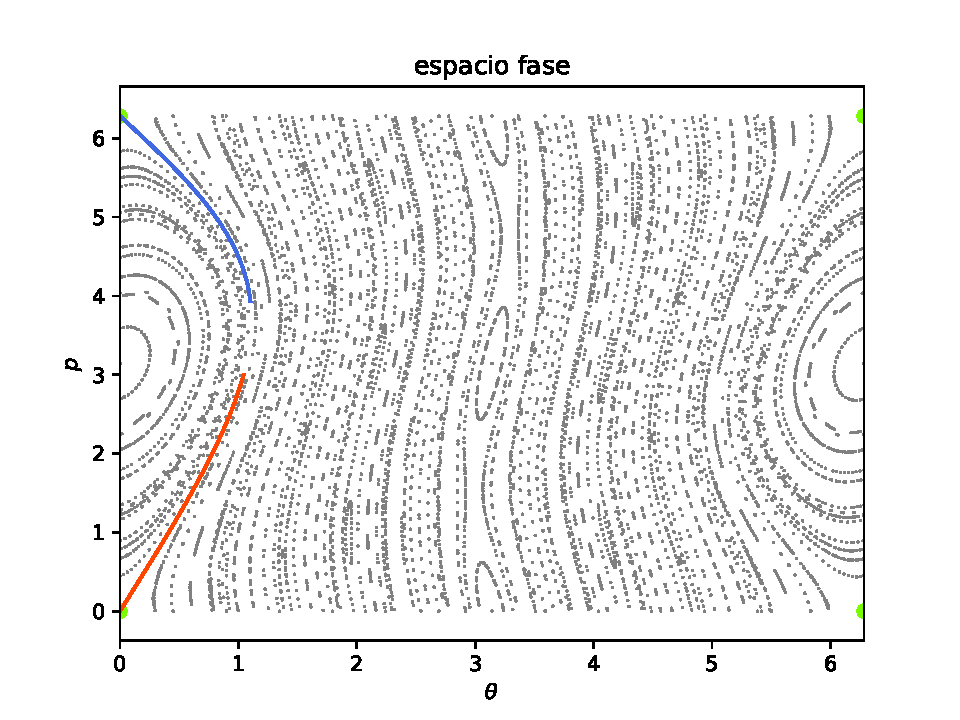
\includegraphics[scale=0.7]{k03}
	\caption{\footnotesize $W^{s},W^{u}$ de orden $25$ en el mapeo estándar con $k=0.3$ en el intervalo $t=[0.,3.]$}
	\label{estandar03}
\end{figure}

\begin{figure}[H]
	\centering
	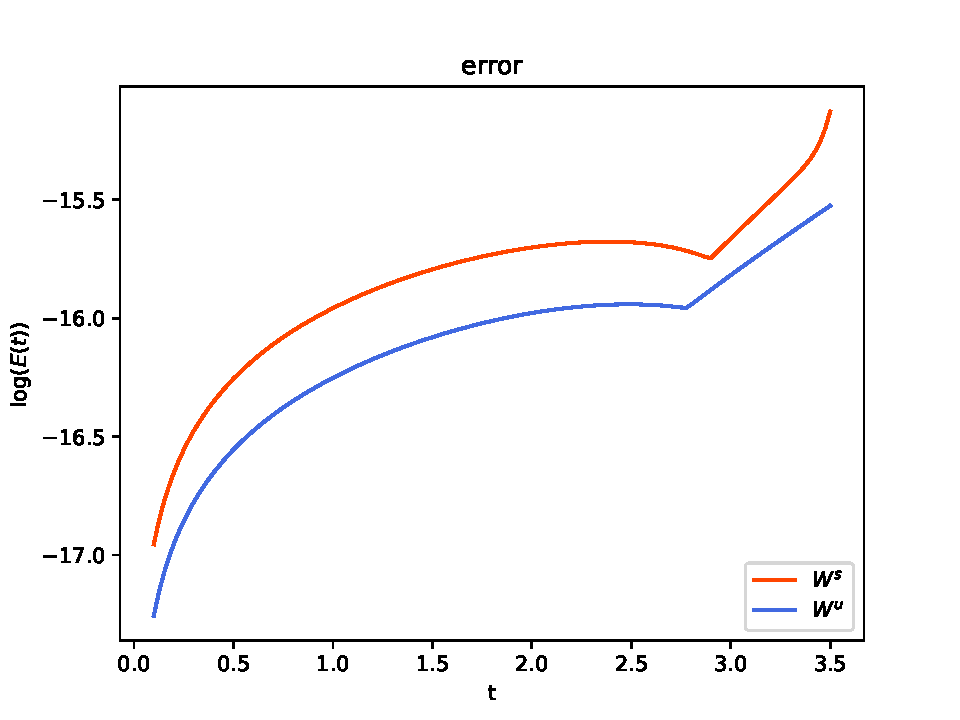
\includegraphics[scale=0.7]{errork03} 
	\caption{Error en las variedades de la figura \ref{estandar03}.}
	\label{error est k03}
\end{figure}


\begin{figure}[H]
	\centering
	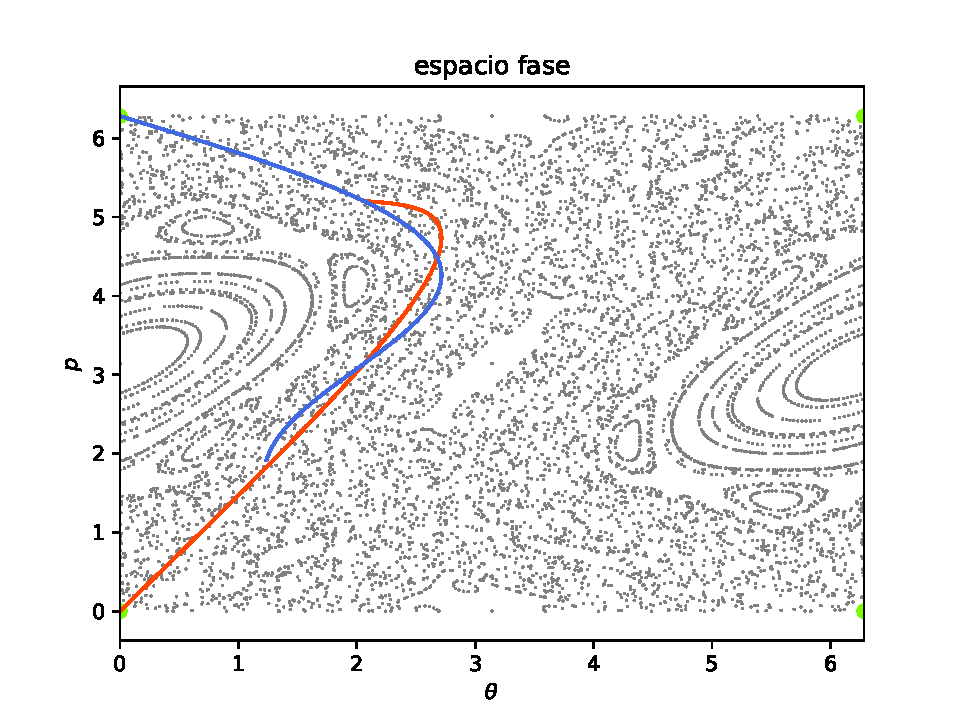
\includegraphics[scale=0.7]{k15}
	\caption{$W^{s},W^{u}$ de orden $80$ en el mapeo estándar con $k=1.5$ en el intervalo $t=[0.,13.].$}
	\label{estandar15}
\end{figure}

\begin{figure}[H]
	\centering
	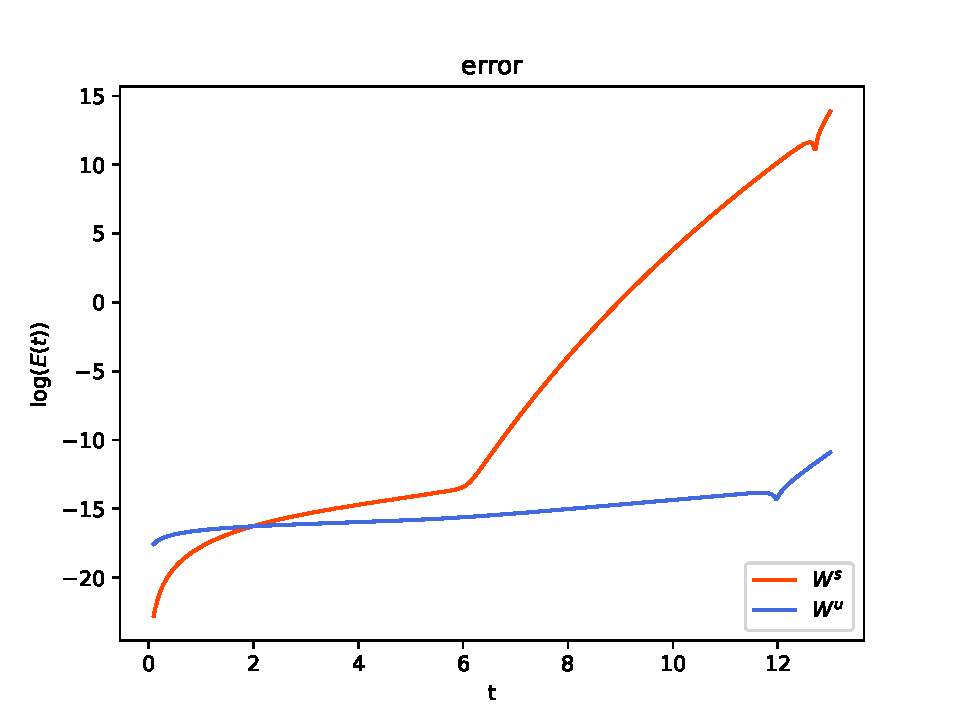
\includegraphics[scale=0.7]{errork15} 
	\caption{Error en las variedades de la figura \ref{estandar15}.}
	\label{error est k15}
\end{figure}




\begin{figure}[H]
	\centering
	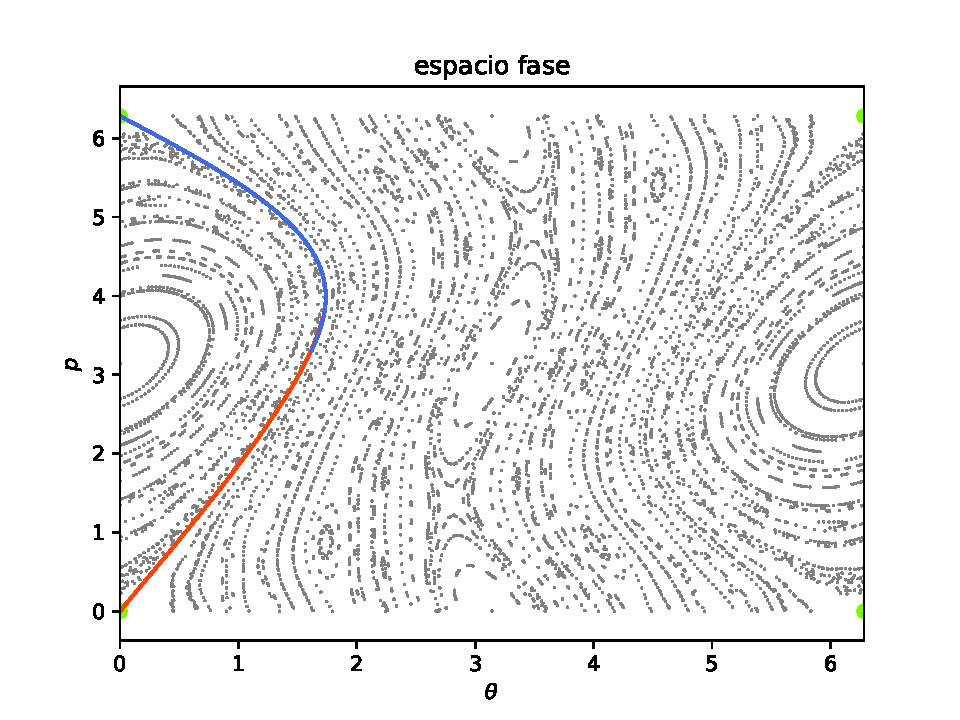
\includegraphics[scale=0.7]{k07}
	\caption{$W^{s},W^{u}$ de orden 70 en el mapeo estándar con $k=0.7$ en el intervalo $t=[0.,5.5]$.}
	\label{estandar07}
\end{figure}

\begin{figure}[H]
	\centering
	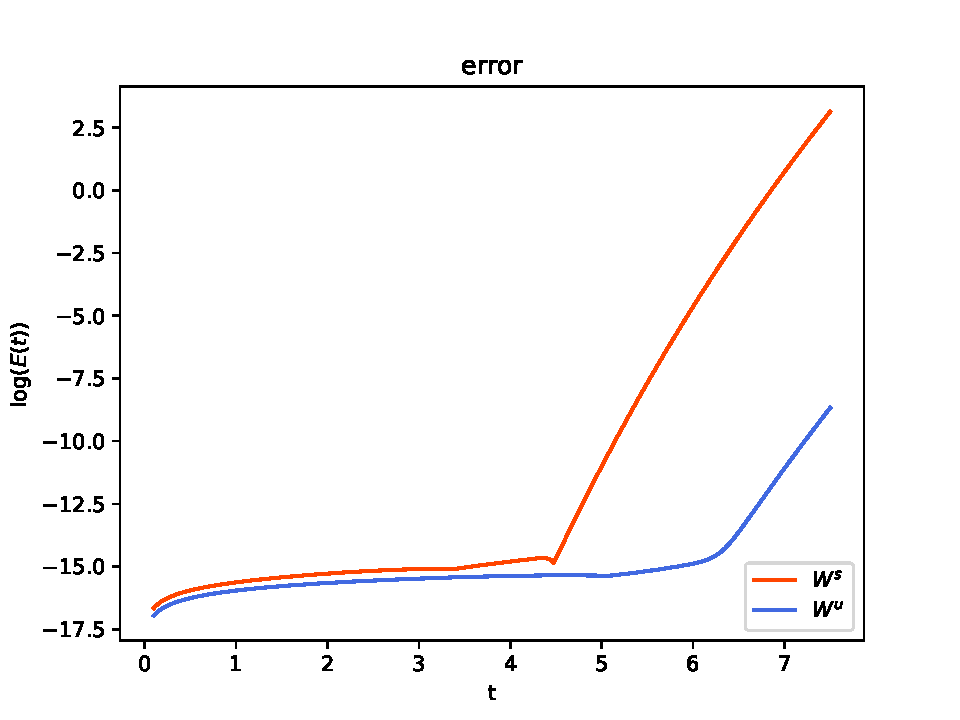
\includegraphics[scale=0.7]{errork07} 
	\caption{Error en las variedades de la figura \ref{estandar07}.}
	\label{error est k07}
\end{figure}



Para observar cómo cambia el comportamiento del error respecto al orden de la parametrización se calcularon polinomios de diferente orden que parametrizan a la variedad inestable del mapeo con $k=0.3$, como se muestra en la figura \ref{erroresf64}. Se observa que mientras más grande sea el orden del polinomio, mejor es la aproximación, pues es posible llegar a valores del parámetro más grandes, que se traduce en ir más lejos en la variedad inestable. \\

\begin{figure}[H]
\centering
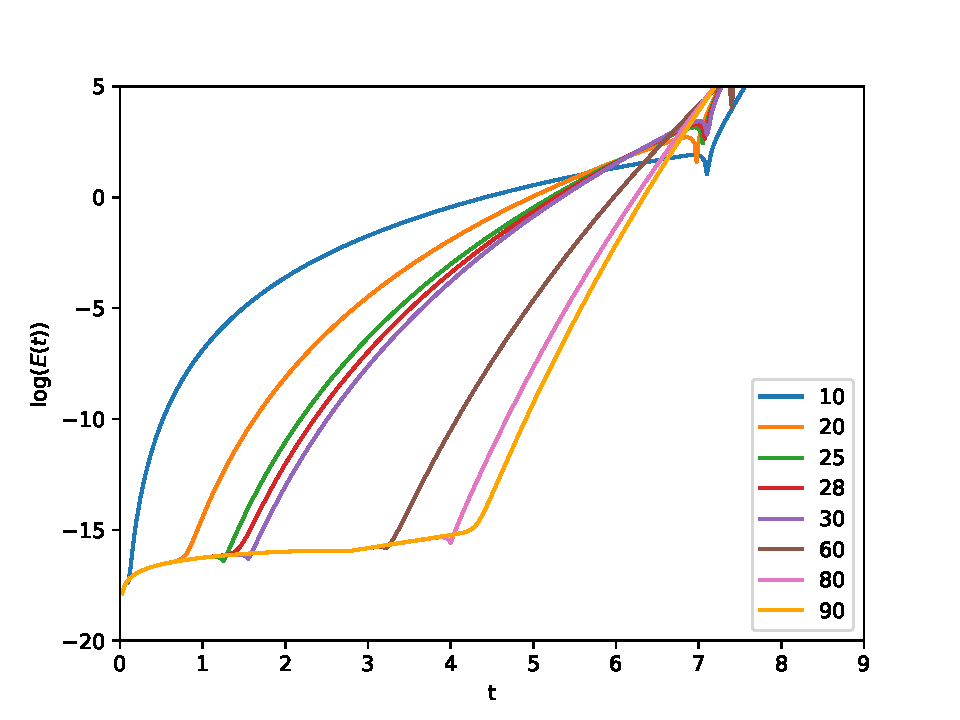
\includegraphics[scale=0.7]{errorf64}
\caption{Curvas de error para diferentes órdenes en el mapeo estándar, $k=0.3$. }
\label{erroresf64}
\end{figure}
A fin de mostrar que el error es de alguna manera controlable se usaron números de precisión extendida (256 bits) para hacer cálculos análogos a los anteriores. En la figura \ref{erroresBig} se muestran los resultados para parametrizaciones de órdenes entre $10$ y $80$. Se observa un comportamiento análogo, de tal manera que para cada orden diferente de parametrización hay un valor diferente del parámetro en el cual pasa de un error que no crece significativamente a un error que crece de manera abrupta. También se notó que al usar precisión extendida(256 bits, $\epsilon_{\mathrm{mach}}=10^{-77}$) el error cerca del punto fijo es imperceptible pero en la parte donde crece, tiene un cambio más pronunciado que en el caso de números de punto flotante. 

\begin{figure}[H]
\centering
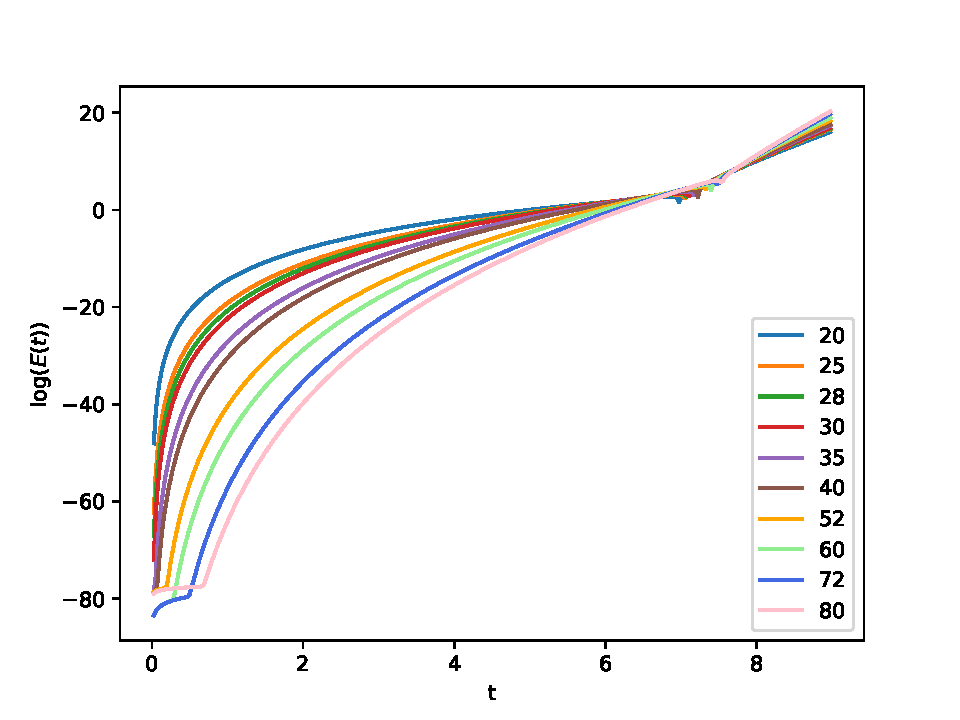
\includegraphics[scale=0.7]{errorbf}
\caption{Curvas de error para diferentes órdenes usando precisión extendida ,$k=0.3$. }
\label{erroresBig}
\end{figure}

Como ya se mencionó antes, la variedad inestable del mapeo inverso corresponde a la variedad estable del mapeo. Si se usa el mismo método calculando la variedad inestable del mapeo inverso \eqref{mapeo estandar inverso} se puede controlar mejor el error numérico. Para mostrar esto se hizo una comparación parametrizando la variedad estable mediante el mapeo inverso y el mapeo inicial. Los polinomios fueron del mismo orden y lo que se observa en el error se muestra en la figura \ref{erroresinverso}.


\begin{figure}[H]
\centering
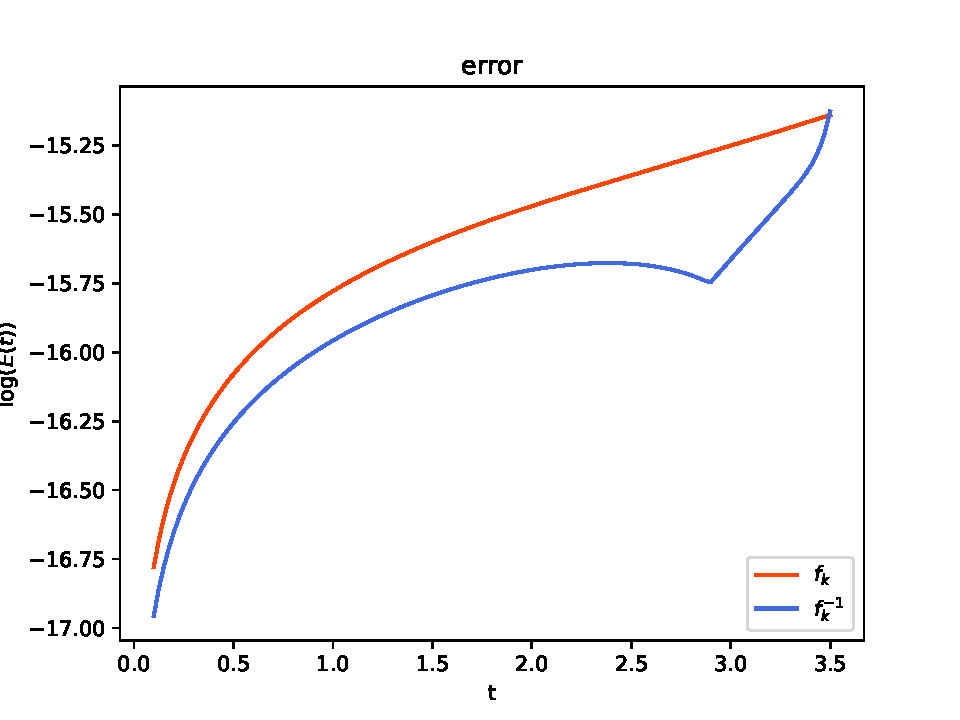
\includegraphics[scale=0.7]{error_inversa}
\caption{Error para las parametrizaciones usando el mapeo y el mapeo inverso con polinomios de orden $20$ y $k=0.3$. }
\label{erroresinverso}
\end{figure}

Usar el mapeo inverso para calcular la variedad estable resulta ser mejor que usar el mapeo normal. El error se mantiene casi sin cambios hasta una valor de $t$ mayor en el caso del mapeo inverso. 




\label{henon-seccion}\section{Mapeo de Hénon}
El mapeo de Hénon se define como \cite{devaney}
\begin{eqnarray}
\mathbf{f}_{a,b}(x,y)=\left( \begin{array}{lcc}
             a-by-x^{2}\\
             \\ x
             \end{array}
             \right), \label{Henon}
\end{eqnarray}

siendo el mapeo inverso
\begin{eqnarray}
\mathbf{f}^{-1}_{a,b}(x,y)=\left( \begin{array}{lcc}
             y\\
             \\ (a-x-y^{2})/b
             \end{array}
             \right). \label{HenonI}
\end{eqnarray} 

       
Para poder analizarlo se debe linealizar el sistema. Primero se obtiene el jacobiano 
            
\begin{eqnarray}
D\mathbf{f}_{a,b}(x,y)= \left( \begin{array}{lcc}
                -2x & -b\\
                \\ 1 & 0
                \end{array}
                \right).
                \label{jacobiano-henon}
\end{eqnarray}

                
Puede notarse que en \eqref{jacobiano-henon} el determinante del jacobiano no es igual a uno, sino $\det(D\mathbf{f}_{a,b}(x,y))=b$.
El determinante es constante, entonces será Hamiltoniano en el caso en que $b$ sea igual a uno o menos uno. Para analizar estos casos, se calculan los puntos fijos
\begin{eqnarray}
\mathbf{f}_{a,b}(x,y)=\left( \begin{array}{lcc}
               a-by-x^{2}\\
               \\ x
               \end{array}
               \right) = \left(\begin{array}{lc}
               x \\
               \\ y
               \end{array}
               \right),
\end{eqnarray}        
lo que implica que $a-by-x^{2}=x$ y $x=y$ de donde es claro que la primer ecuación queda
\begin{eqnarray*}
x^{2}+(b+1)x-a=0, 
\end{eqnarray*}
que se puede resolver usando la fórmula general
\begin{eqnarray*}
x=\frac{-(b+1)\pm ((b+1)^{2}+4a)^{1/2} }{2}.
\end{eqnarray*}
Para el caso en que $b=1$ se tiene
\begin{eqnarray}
x=\frac{-2\pm 2(1+a)^{1/2} }{2}.
\end{eqnarray}
Al escoger $b=1$ se garantiza estar en un sistema Hamiltoniano, mientras que $a$ debe escogerse de manera que resulten puntos fijos hiperbólicos $(a>-1)$. La figura \ref{Henon1} muestra un ejemplo de cálculos de variedades para el mapeo de Hénon con $a=1.5$ y polinomios de orden 45, tomando un valor máximo del parámetro $t=1000.0$. El error asociado a la parametrización de la figura \ref{Henon1} se muestra en la figura \ref{ErrorHenon1}; a partir de este punto se usará la notación $W_{f}^{u}$ para denotar la parametrización de la variedad inestable calculada con el mapeo, y $W_{f^{-1}}^{u}$ para denotar la variedad estable calculada con el mapeo inverso.

\begin{figure}[H]
\centering
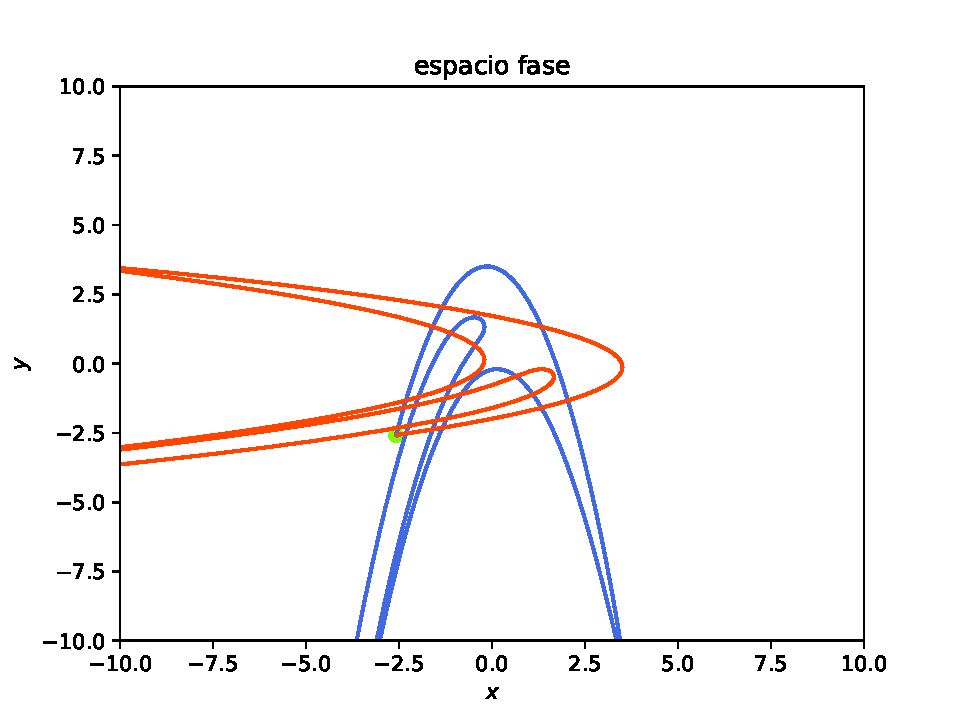
\includegraphics[scale=0.7]{h15}
\caption{$W^{u}$ y $W^{s}$ de orden 45 en el intervalo $t=[0.,900.]$ para el mapeo de Hénon con $a=1.5$,$b=1$.}
\label{Henon1}
\end{figure}

\begin{figure}[H]
\centering
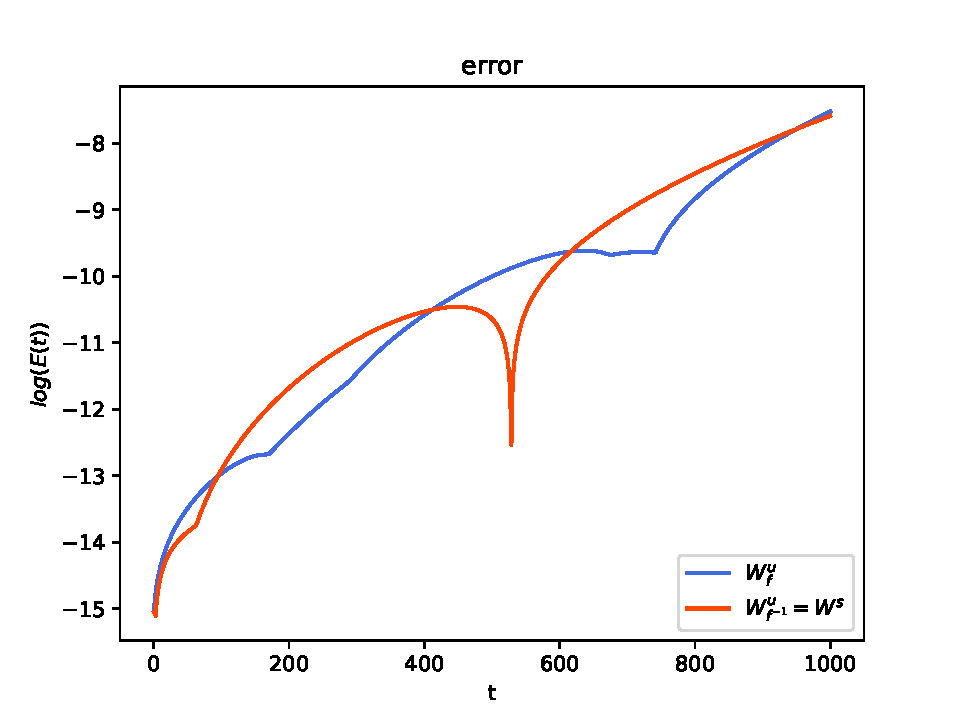
\includegraphics[scale=0.7]{errorH15}
\caption{Error asociado a las variedades de la figura \ref{Henon1}.}
\label{ErrorHenon1}
\end{figure}
Las variedades que aparecen en la figura \ref{Henon1} se calcularon con el mapeo de Hénon \eqref{Henon} y el mapeo inverso \eqref{HenonI}; las variedades se observan simétricas; aún así, las parametrizaciones son diferentes. Puede verse en la figura \ref{ErrorHenon1} que el error cambia cinco órdenes de magnitud en todo el intervalo del parámetro.\\

A diferencia del mapeo estándar, en este mapeo las órbitas pueden escapar a infinito, es decir, no están  constreñidas en una región finita, lo que representa un mayor reto en cuanto a la parametrización, ya que el polinomio debe ser tal que pueda regresar varias veces. De hecho se observa que son necesarios valores grandes en el parámetro, comparados con los del mapeo estándar, para observar los cruces de las variedades. También esta situación hace que el error numérico sea mayor que para el mapeo estándar. \\

En las figuras \ref{Henon2}, \ref{Henon3} se muestran las variedades calculadas de la misma manera en la que se calcularon para la figura \ref{Henon1}. En \ref{Henon2} las curvas son más cerradas y se necesita de un polinomio de orden mayor que en el caso de \ref{Henon3} para observar los cortes. 
\begin{figure}[H]
\centering
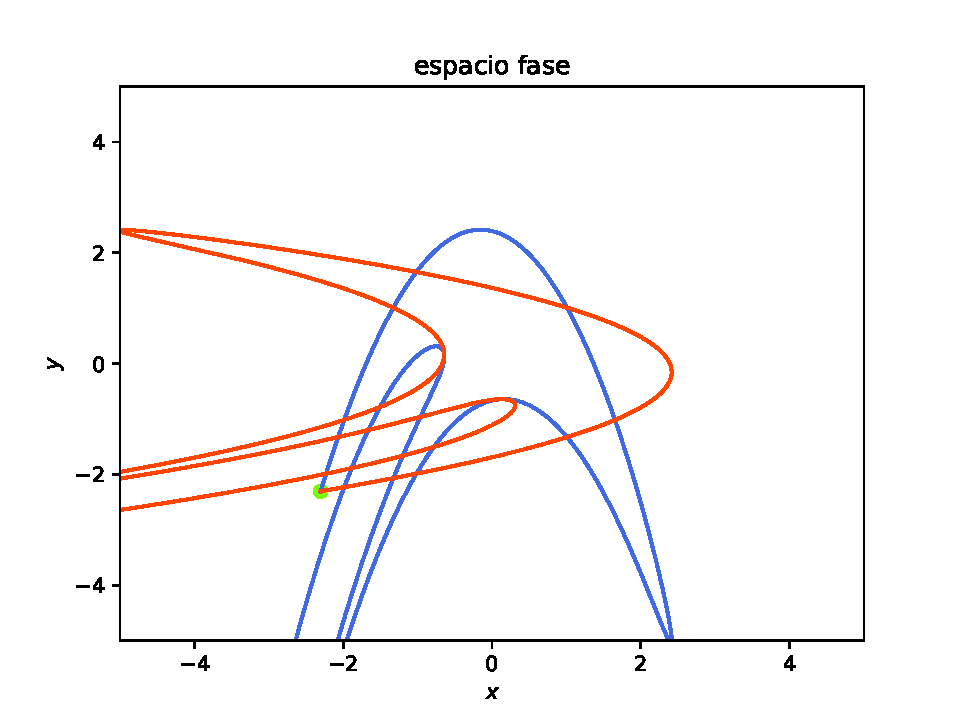
\includegraphics[scale=0.7]{h07}
\caption{$W^{u}$, $W^{s}$ de orden $50$ en el intervalo $t=[0.,800.]$ para el mapeo de Hénon con $a=0.7$,$b=1.$}
\label{Henon2}
\end{figure}

\begin{figure}[H]
\centering
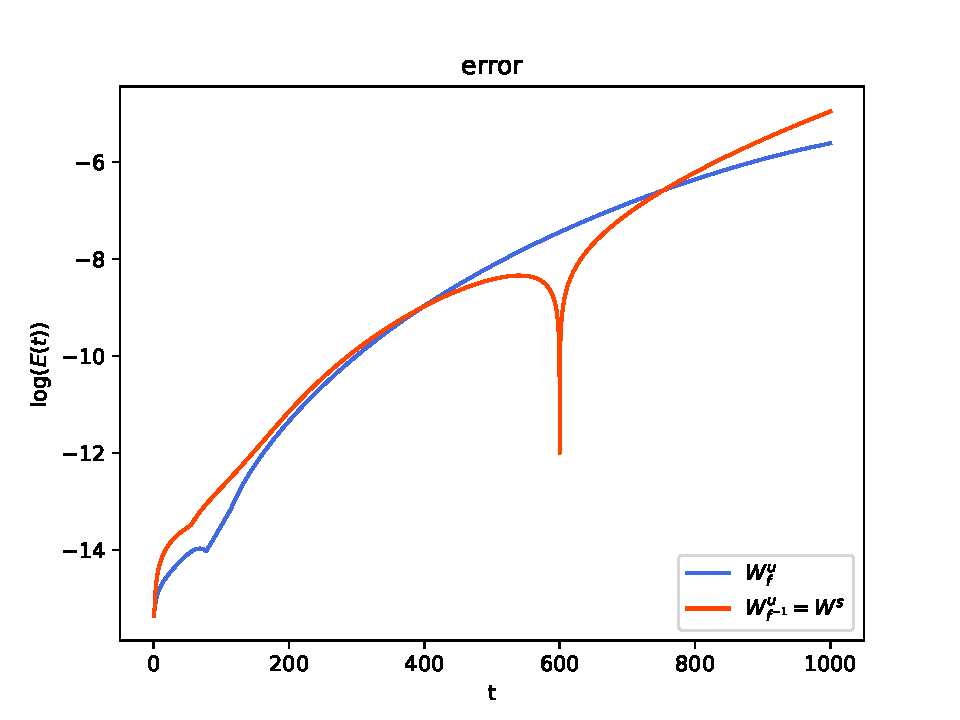
\includegraphics[scale=0.7]{errorH07}
\caption{Error asociado a las variedades de la figura \ref{Henon2}.}
\label{ErrorHenon2}
\end{figure}


\begin{figure}[H]
\centering
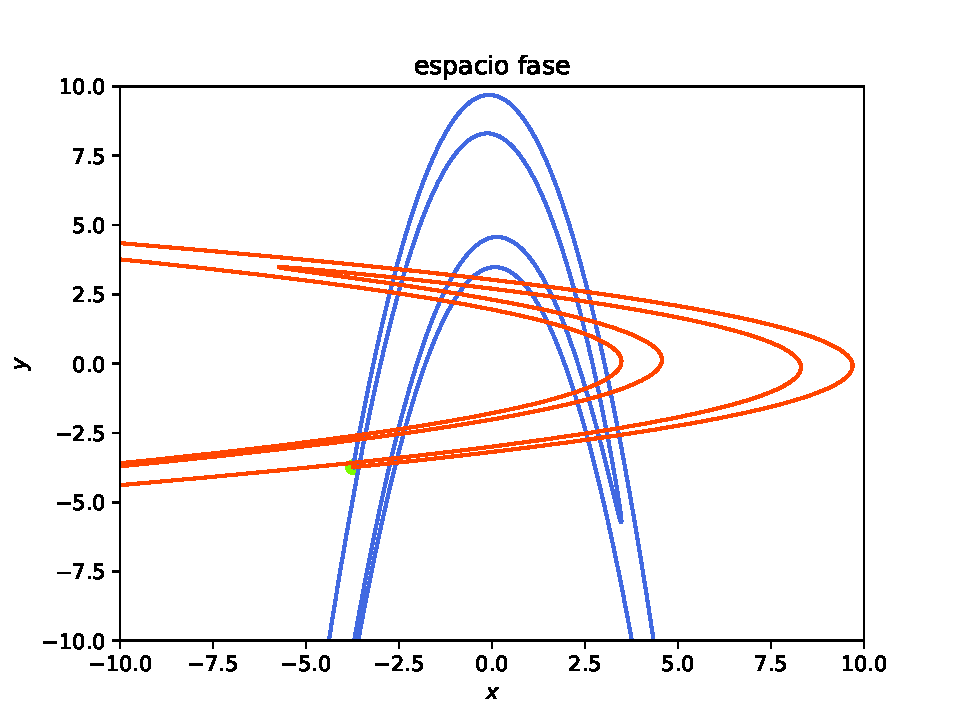
\includegraphics[scale=0.7]{h65}
\caption{$W^{u}$, $W^{s}$ de orden $78$ en el intervalo $t=[0.,4000.0]$ para el mapeo de Hénon con $a=6.5$,$b=1.$.}
\label{Henon3}
\end{figure}

\begin{figure}[H]
\centering
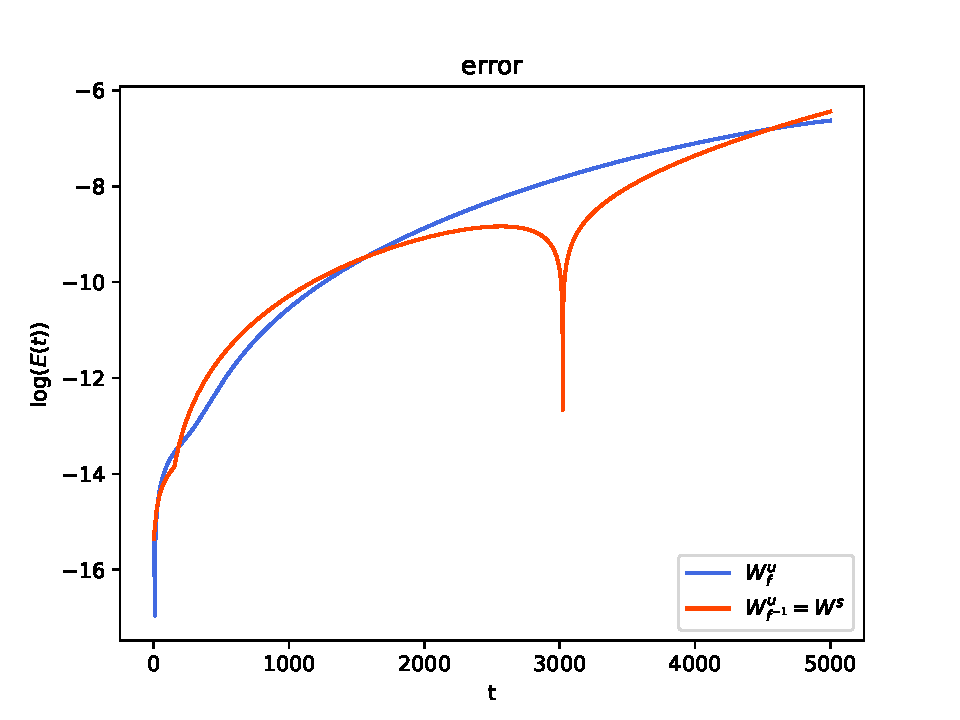
\includegraphics[scale=0.6]{errorH65}
\caption{Error asociado a las variedades de la figura \ref{Henon3}.}
\label{ErrorHenon3}
\end{figure}


Así que con el orden suficiente es posible observar los cruces de ambas variedades; estos cruces son importantes en la dinámica pues dan información sobre caos en el sistema,  en la última sección se habla un poco sobre esto. 

\label{jung-seccion}\section{Mapeo exponencial}
El último mapeo que se estudió fue uno usado en el artículo \citep{Jung}: 
\begin{eqnarray}
\mathbf{j}_{a}(x,y)=\left(\begin{array}{lcc}
             x+y\\
             \\ y+af(x+y)
             \end{array}\right),
\label{Jung}
\end{eqnarray}
que describe el movimiento de una partícula pateada, donde la coordenada $x$ representa la posición en una dimensión, mientras que la coordenada $y$ es el momento; $a$ es un parámetro libre. La función $f$ es la responsable de describir la fuerza aplicada; en el artículo \cite{Jung} se escoge
\begin{eqnarray*}
f(x)=x(x-1)e^{-x}.
\end{eqnarray*}
A este mapeo le corresponde su mapeo inverso
\begin{eqnarray}
\mathbf{j}^{-1}_{a}(x,y)=\left(\begin{array}{lcc}
             x-y+ax(x-1)e^{-x}\\
             \\ y-ax(x-1)e^{-x}
             \end{array}\right).
             \label{jungI}
\end{eqnarray}
Los puntos fijos del sistema son $\mathbf{x}_{0}=(1,0), \mathbf{x}_{1}=(0,0)$; $\mathbf{x}_{0}$ es un punto fijo hiperbólico. El punto $\mathbf{x}_{1}$ es un punto elíptico mientras el valor del parámetro $a$ sea menor a 4, y para valores de $a \geq 4$ se torna inverso hiperbólico.\\

Usando el mismo procedimiento que en los casos anteriores se obtuvieron las figuras \ref{jung1}--\ref{errorjung2}, que muestran cómo se comportan las variedades aún en el caso en que el sistema no sea completamente hiperbólico. Como en los casos anteriores el error asociado a la variedad estable es mayor, después de cierto valor del parámetro, que el asociado a la variedad inestable. El orden al que se debe llegar en los polinomios para observar algunos de los cortes de las variedades es más alto en comparación con el mapeo de Hénon, debido a que en el caso del mapeo exponencial se está aproximando una función exponencial.

\begin{figure}[H]
\centering
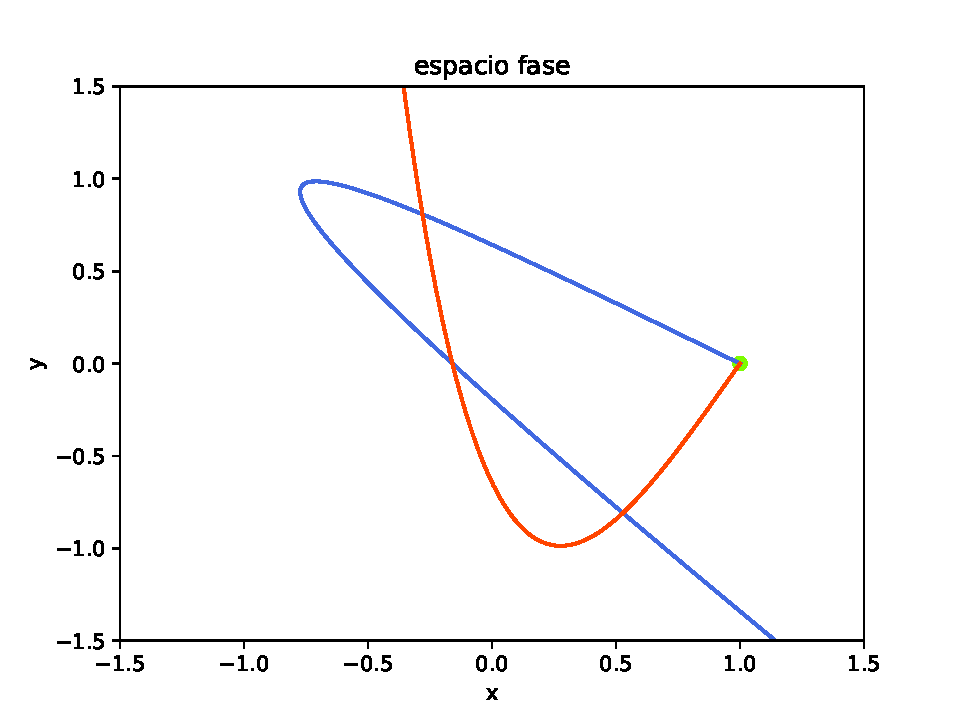
\includegraphics[scale=0.7]{jung34}
\caption{$W^{s}$ y $W^{u}$ de orden 86 en el intervalo $t=[0.,5.5]$, con $a=3.4$, en el punto fijo $x_{0}$.}
\label{jung1}
\end{figure}

\begin{figure}[H]
\centering
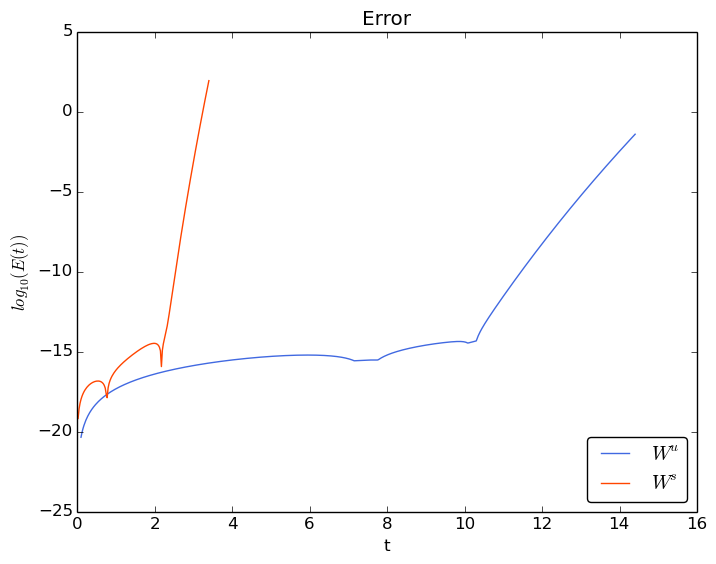
\includegraphics[scale=0.7]{error_jung34}
\caption{Error asociado a las variedades de la figura \ref{jung1}.}
\label{errorjung1}
\end{figure}


\begin{figure}[H]
\centering
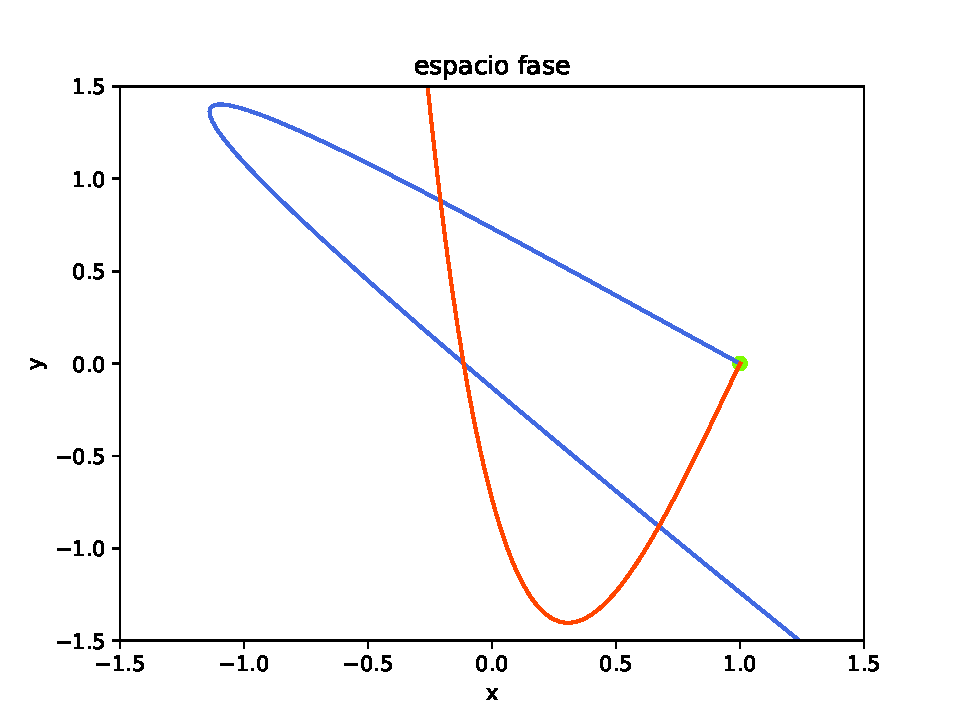
\includegraphics[scale=0.7]{jung57}
\caption{$W^{s}$ y $W^{u}$ de orden 93 en el intervalo $t=[0.,6.5]$, con $a=5.7$ en el punto fijo $x_{0}$.}
\label{jung2}
\end{figure}


\begin{figure}[H]
\centering
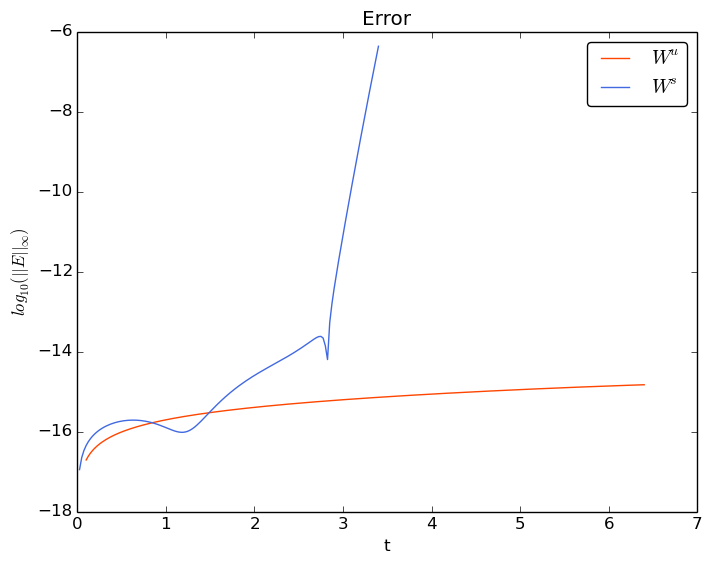
\includegraphics[scale=0.7]{error_jung57}
\caption{Error asociado las variedades de la figura \ref{jung2}.}
\label{errorjung2}
\end{figure}
Se puede observar en las figuras \ref{errorjung1}, \ref{errorjung2} que en la variedad estable el error crece de manera abrupta antes que el error de la variedad inestable. Ambas curvas del error tienen la misma forma, y se mantienen aproximadamente en el mismo orden de error. El mapeo \eqref{Jung} es más sensible que los dos mapeos pasados, algunos órdenes resultaban no ajustarse a la variedad más allá de valores del parámetro menor a uno.\\



\section{Convergencia}
Además de medir el error asociado a la parametrización se consideró importante tomar en cuenta la convergencia de los coeficientes de los polinomios. En casos como el mapeo exponencial en que las variedades se acercan a puntos fijos de diferente naturaleza puede ocurrir que tal cercanía afecte la forma de parametrización. Para ello se implementaron dos formas de revisar la convergencia, la de Hadamard \eqref{hadamard} y la de tres términos \eqref{tres terminos}. \\

La figura \ref{convergenciaEst15} muestra la convergencia de los polinomios de orden 25 que parametrizan la variable $\theta$ en el mapeo estándar para las variedades estable e inestable con $k=1.5$, a la que corresponde el espacio fase mostrado en la figura \ref{estandar15}. En ambos casos se ve que los coeficientes cambian de manera suave y se van haciendo cada vez más pequeños comparados con el anterior; se dice entonces que los coeficientes de la parametrización convergen a cero.  
\begin{figure}[H]
\centering
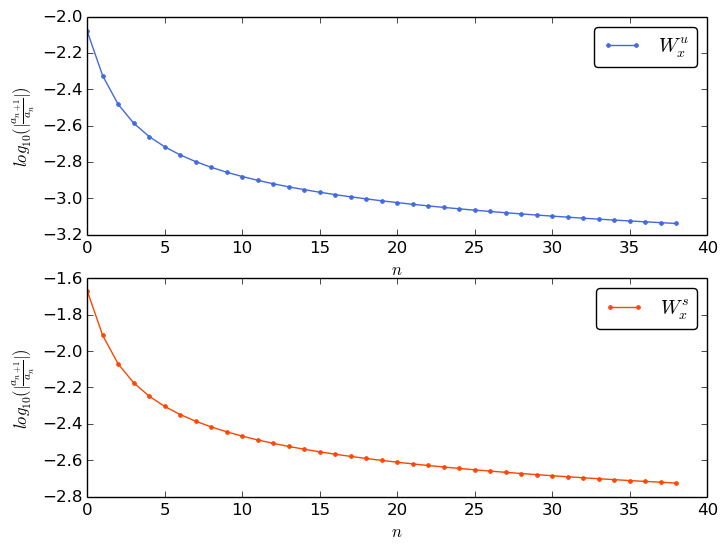
\includegraphics[scale=0.8]{converEst15}
\caption{Convergencia de Hadamard asociada a los polinomios para $\theta$ en las variedades del mapeo estándar con $k=1.5$. Con $n\in\mathbb{Z}$.}
\label{convergenciaEst15}
\end{figure}

La figura \ref{convergenciaHenon1} muestra la convergencia de las parametrizaciones de orden 45 para la variable $x$ en el mapeo de Hénon con $a=1.5$. En ambos casos la convergencia parece suave y tiende a cero igual que en el caso del mapeo estándar.

\begin{figure}[H]
\centering
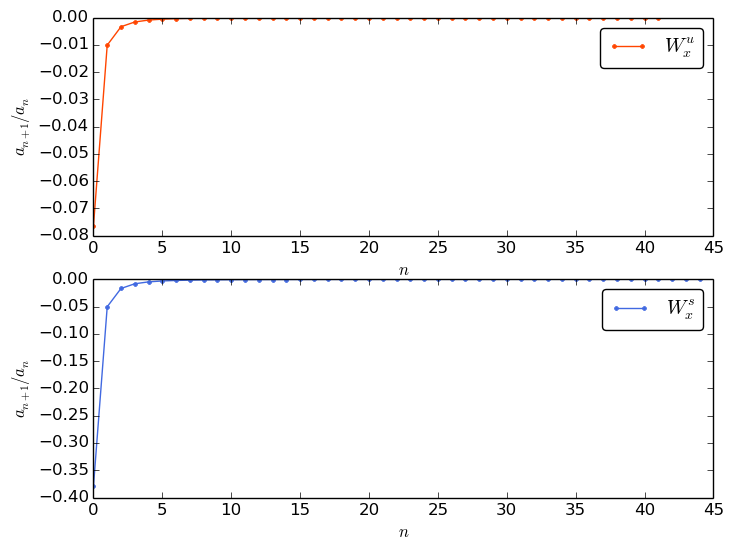
\includegraphics[scale=0.8]{converHenon1}
\caption{Convergencia de Hadamard asociada a los polinomios para $x$ en las variedades del mapeo de Hénon con $a=1.5$. Con $n\in\mathbb{Z}$.}
\label{convergenciaHenon1}
\end{figure}


Para el mapeo exponencial se realizaron los dos criterios de convergencia. La figura \ref{convergenciaJH} muestra el criterio de Hadamard \eqref{hadamard}: para los polinomios que parametrizan la variable $x$ en cada variedad, se ve que hay una convergencia clara de los coeficientes en el caso de la variedad inestable; para el caso de la estable parece que después de cierto orden los coeficientes no convergen. Lo mismo ocurre en la figura \ref{convergenciaJ3} en donde se usó el criterio de tres términos \eqref{tres terminos}, con $C_{n}=n\left(\frac{a_{n+1}}{a_{n}}\right)-(n-1)\left(\frac{a_{n}}{a_{n-1}}\right)$.

\begin{figure}[H]
\centering
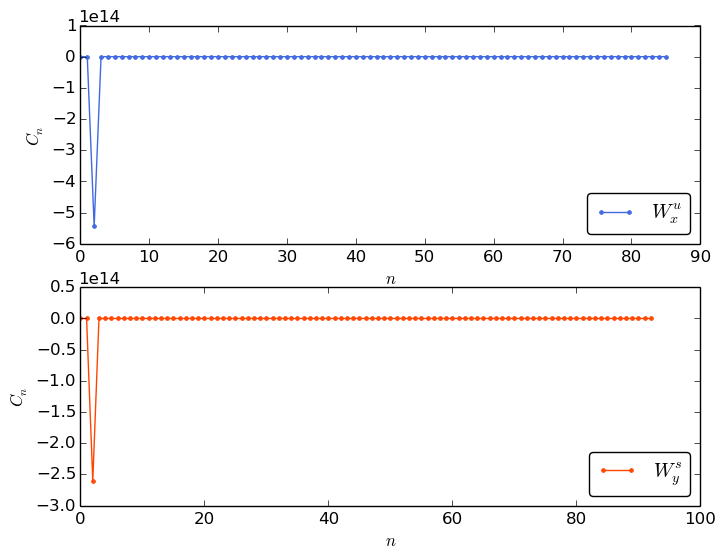
\includegraphics[scale=0.7]{convergenciaJungH57}
\caption{Convergencia de Hadamard asociada a las variedades mostradas en la figura \ref{jung2}.}
\label{convergenciaJH}
\end{figure}


\begin{figure}[H]
\centering
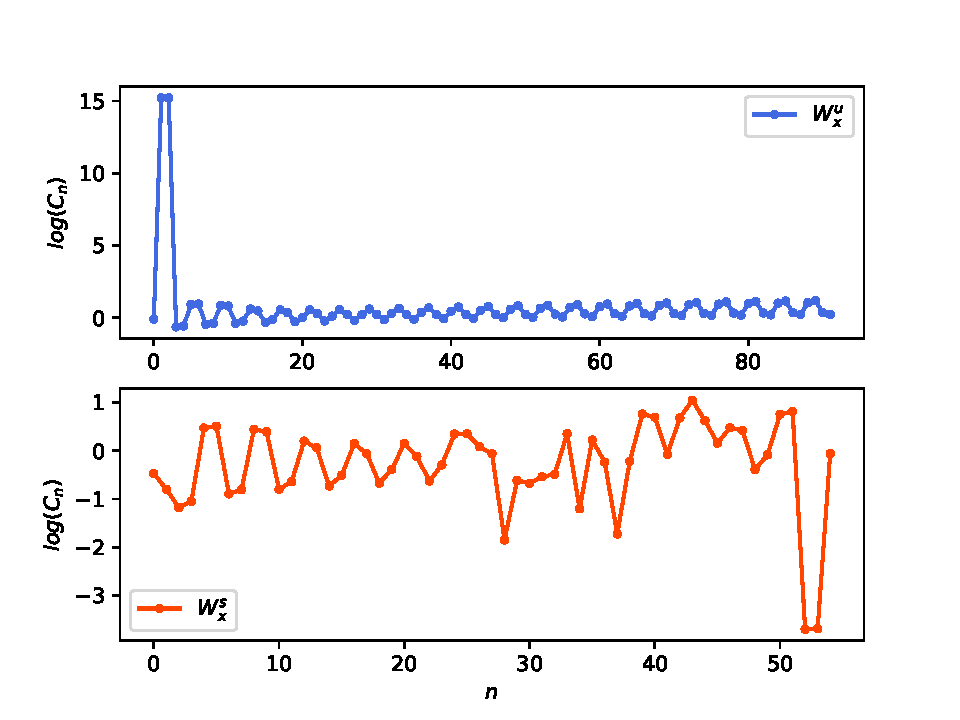
\includegraphics[scale=0.7]{convergenciaJungT57}
\caption{Convergencia de tres términos asociada a las variedades en la figura \ref{jung2}.}
\label{convergenciaJ3}
\end{figure}

Estudiar la convergencia de las parametrizaciones puede dar una idea de cómo se va modificando el polinomio si se cambia el orden, en mapeos más sensibles puede ser determinante para saber a qué orden es conveniente aproximar. 

\section{Existencia de puntos homoclínicos/heteroclínicos}

Siendo que el resultado son polinomios, se puede aplicar el método de Newton, o cualquier otro, en dos dimensiones para resolver $\mathcal{P}^{u}=\mathcal{P}^{s}$, encontrando puntos homoclínicos o heteroclínicos. Por suerte existe una paquetería en Julia que hace cálculos numéricos validados, \texttt{ValidatedNumerics} \cite{validated} dentro de la cual se tiene un paquete para aritmética de intervalos, \texttt{IntervalArithmetic} \citep{interval}, y otro para encontrar raíces, \texttt{IntervalRootFinding} \cite{root}.\\

El paquete \cite{validated} hace cálculos de computación rigurosa con números de punto flotante usando el paquete de aritmética de intervalos, que efectúa operaciones con intervalos en lugar de números, mientras que \cite{root} automatiza métodos populares como el de Newton para encontrar raíces de funciones; en este caso se garantiza que la respuesta correcta se encuentra en un intervalo. Para entender mejor cómo funcionan cada una de las paqueterías, así como la teoría rigurosa detrás de éstos,se recomienda revisar \cite{ramon}, \cite{Numerics}. Dicho de manera breve, los paquetes ya mencionados generalizan las operaciones y funciones en términos de conjuntos, de tal manera que la solución contenga la respuesta correcta. \\

Las variedades parametrizadas que resultan del método son polinomios, por lo que con las paqueterías  mencionadas se puede analizar cuando dos de ellas se cruzan. Concretamente se tienen  $W^{s}(t)=(\mathcal{P}_{x}(t),\mathcal{P}_{y}(t))$ y $W^{u}(\tau)=(\mathcal{P}_{x}(\tau),\mathcal{P}_{y}(\tau))$ de órdenes no necesariamente iguales, y se busca que:
\begin{eqnarray}
W^{s}(t)=W^{u}(\tau),
\end{eqnarray}
que arrojará como resultado un intervalo $I_{t}$ y otro intervalo $I_{\tau}$, tal que la intersección se encontrará en $I_{t}\times I_{\tau}$. En el espacio fase la intersección se verá como el producto cartesiano de $W^{s}(I_{t})\times W^{u}(I_{\tau})$ formando una sección en la que se garantiza hay un punto homoclínico o heteroclínico. 


\subsection{Estándar}
Usando lo descrito anteriormente se calcularon las intersecciones de las variedades estable e inestable en el mapeo estándar para un valor de $k=1.5$ usando polinomios de orden $120$, además de usar el mapeo inverso \eqref{mapeo estandar inverso} para calcular la variedad estable. Se encontraron cuatro raíces en el intervalo $[-20.,0.]$ para $t$  y $[-15.,0.]$ para $\tau$, con una tolerancia de $10^{-6}$ usando el método de Newton, las cuales son:
\begin{itemize}
\item Root$([-7.16826, -7.16825] \times [-4.45972, -4.45971]$, :unique)
\item Root$([-4.21757, -4.21756] \times [-8.36029, -8.36028]$, :unique)
\item Root$([-2.24983, -2.24982] \times [-14.2093, -14.2092]$, :unique)
\item Root$([-13.4378, -13.4377] \times [-2.62396, -2.62395]$, :unique)
\end{itemize}
El primer intervalo corresponde al parámetro $t$ mientras que el segundo al parámetro $\tau$; la leyenda \texttt{unique} indica que en el intervalo presentado sólo hay una raíz. Las raíces se representan gráficamente en el espacio fase en la figura \ref{cruce_estandar}. 

\begin{figure}[H]
\centering
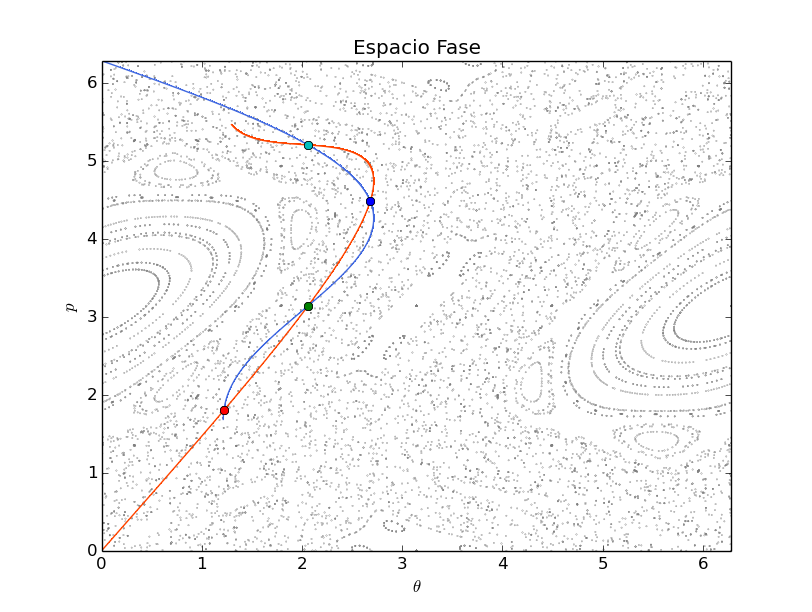
\includegraphics[scale=0.7]{cruce_estandar}
\caption{Cruces de $W^{u},W^{s}$ de orden $120$ para el mapeo estándar con $k=1.5$ .}
\label{cruce_estandar}
\end{figure}
El error asociado al cálculo de las variedades se puede ver en la figura \ref{errorEstCruces}, en dónde se aprecia que los valores aceptables de los parámetros están dentro del intervalo inicial. 

\begin{figure}[H]
\centering
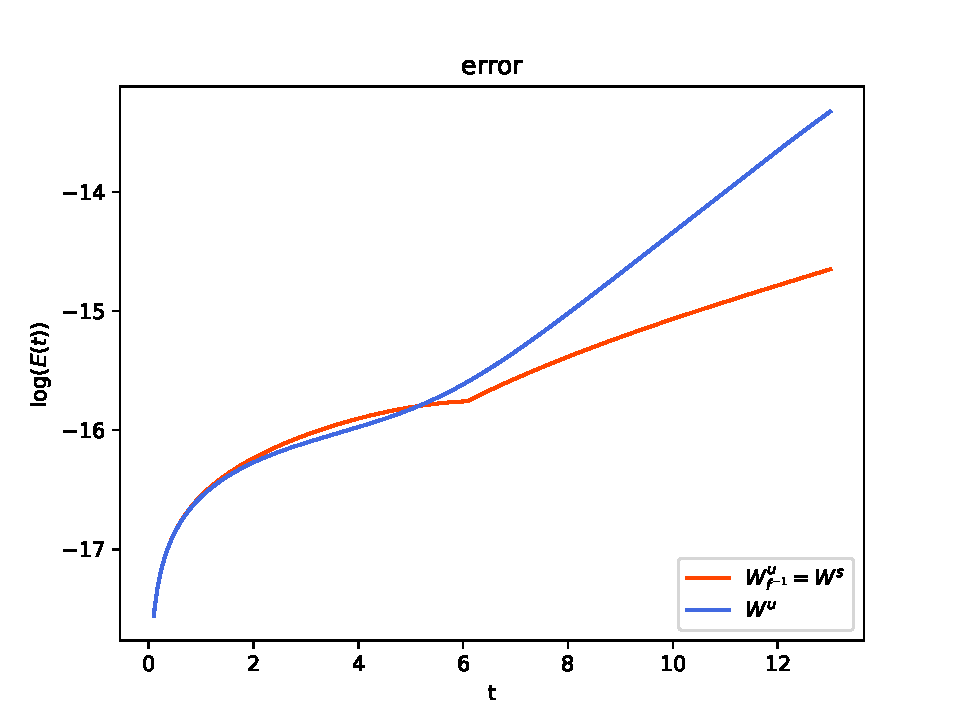
\includegraphics[scale=0.7]{error_cruces_estandar}
\caption{Error en las variedades de la figura \ref{cruce_estandar}.}
\label{errorEstCruces}
\end{figure}

El cálculo numérico riguroso garantiza que la solución está en el intervalo que da como resultado, sin embargo no hay que olvidar: las variedades tienen un error asociado, por lo que es importante quedarse en aquellos intervalos del parámetro donde se tenga un error mínimo; en otras palabras, el método de encontrar raíces está validado mientras que el cálculo de los coeficientes de polinomios no. Con las raíces obtenidas se asegura que en el mapeo estándar con el valor del parámetro $k=1.5$ se encuentran cuatro intersecciones de las variedades, sin embargo es necesaria sólo una de ellas para saber que hay un número infinito\citep{Ott}. Si se quiere encontrar más intersecciones, de manera directa, se debe considerar un polinomio de orden mayor o en todo caso usar números de precisión extendida para llegar más lejos en las variedades. 



\subsection{Hénon}
Así como se calcularon las intersecciones en las variedades del mapeo estándar se calculan para el mapeo de Hénon. En este caso se usó un valor del parámetro $a=1.5$ con un polinomio de orden 65 y el método de Newton con una tolerancia de $10^{-6}$ además de usar el mapeo inverso \eqref{HenonI}, para calcular la variedad estable. Los resultados fueron los siguientes intervalos:
\begin{itemize}
\item[$\alpha$)] Root$([-1.36597, -1.36596] \times [166.749, 166.75]$, :unique)
\item[$\beta$)] Root$([-5.26555, -5.26554] \times [129.577, 129.578]$, :unique)
\item[$\gamma$)] Root$([-6.77613, -6.77612] \times [33.6142, 33.6143]$, :unique)
\item[$\delta$)] Root$([-5.54438e-07, 0] \times [0, 5.54438e-07]$, :unknown)     
\item[$\phi$)] Root$([-26.1208, -26.1207] \times [26.1207, 26.1208]$, :unique)  
\item[$\rho$)] Root$([-33.6143, -33.6142] \times [6.77612, 6.77613]$, :unique)  
\item[$\psi$)] Root$([-129.578, -129.577] \times [5.26554, 5.26555]$, :unique) 
\item[$\eta$)] Root$([-166.75, -166.749] \times [1.36596, 1.36597]4$, :unique)
\end{itemize}

La leyenda \texttt{unknown} dice que no puede concluir nada sobre la intersección en el intervalo. El tercer intervalo $\delta$ contiene al cero $(t,\tau)=(0,0)$ en el cual se cortan las variedades pues representa el punto fijo. La figura \ref{crucesH} representa con un punto los cortes encontrados en las variedades.
\begin{figure}[H]
\centering
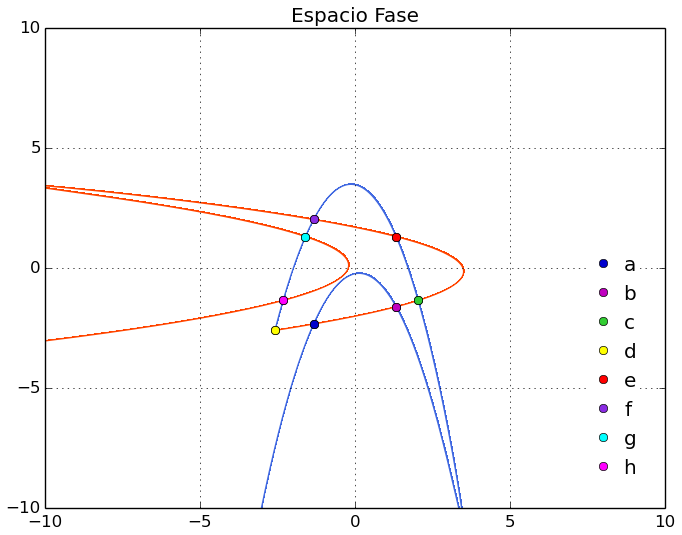
\includegraphics[scale=0.7]{crucesL}
\caption{Cruces de $W^{u},W^{s}$ encontrados en el intervalo $[-400.,0.] \times [0.,400.]$ .}
\label{crucesH}
\end{figure}
Los puntos de color son sólo para indicar cuales intersecciones fueron encontradas. Para los intervalos encontrados se hizo una gráfica que representa la región en el espacio fase donde se encuentra el cruce; la figura \ref{matriz_cortes} muestra cada una de ellas.

\begin{figure}[htbp]
\centering
\subfigure{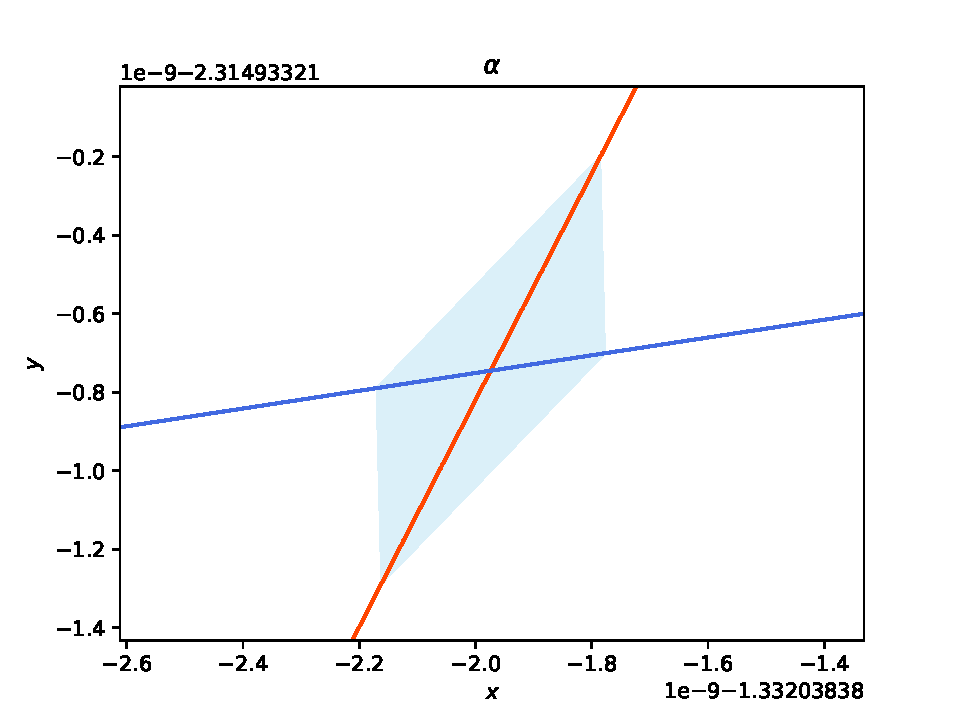
\includegraphics[width=65mm]{alpha}}\hspace{0mm}
\subfigure{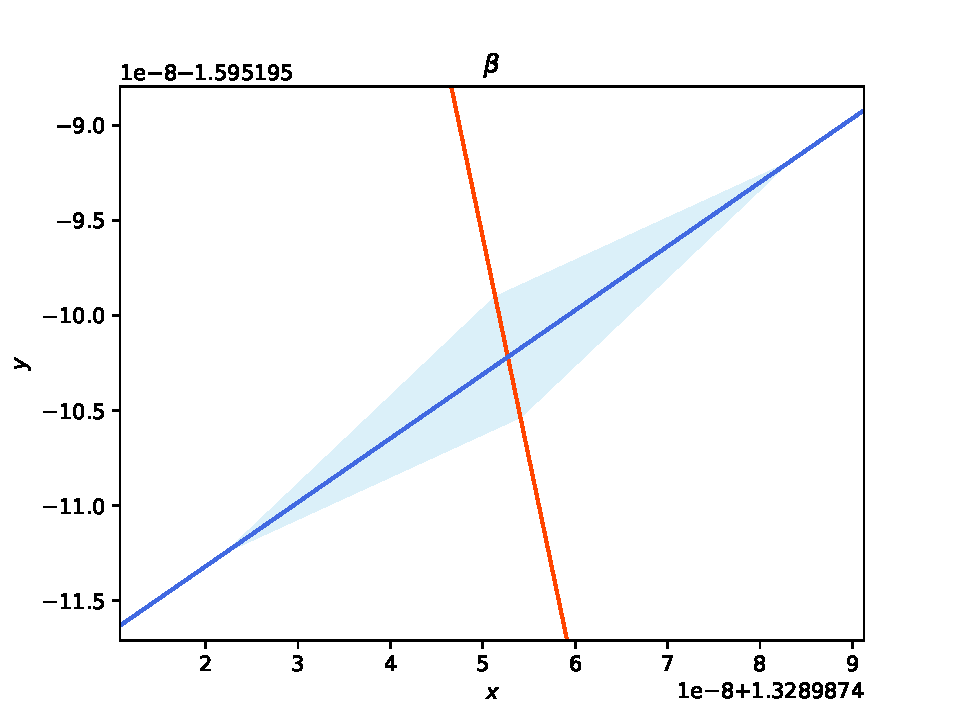
\includegraphics[width=65mm]{beta}}\vspace{0mm}
\subfigure{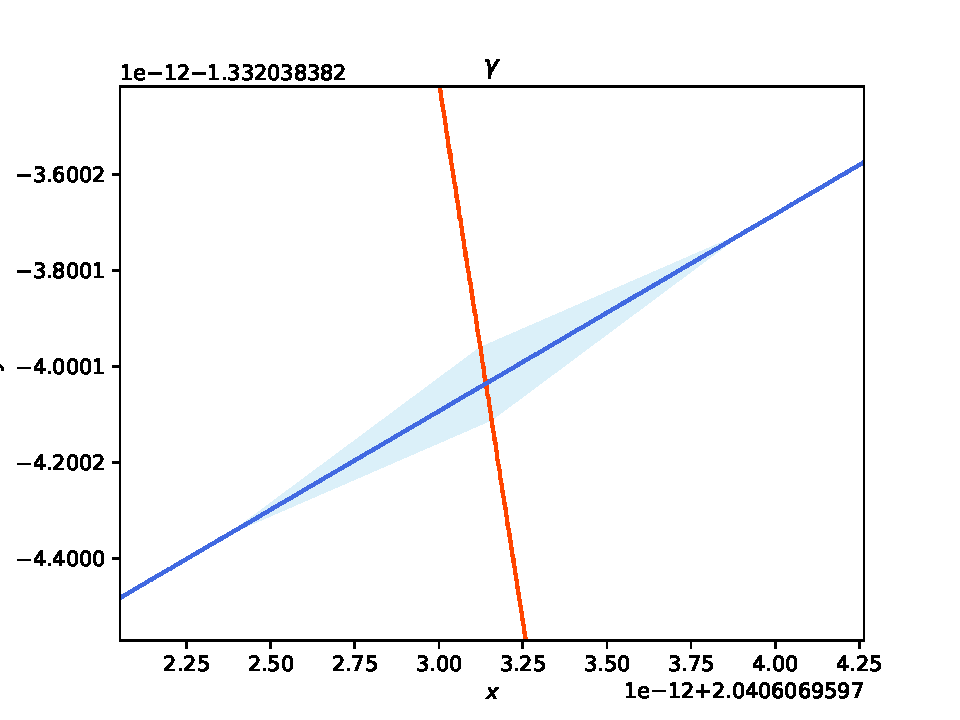
\includegraphics[width=65mm]{gamma}}\hspace{0mm}
\subfigure{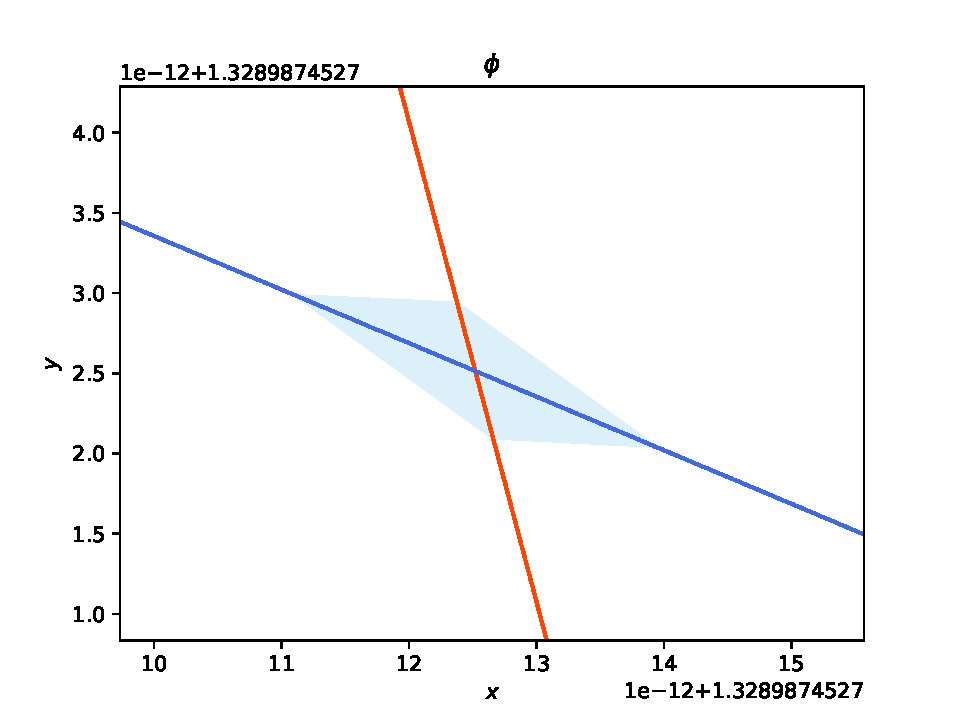
\includegraphics[width=65mm]{phi}}\vspace{0mm}
\subfigure{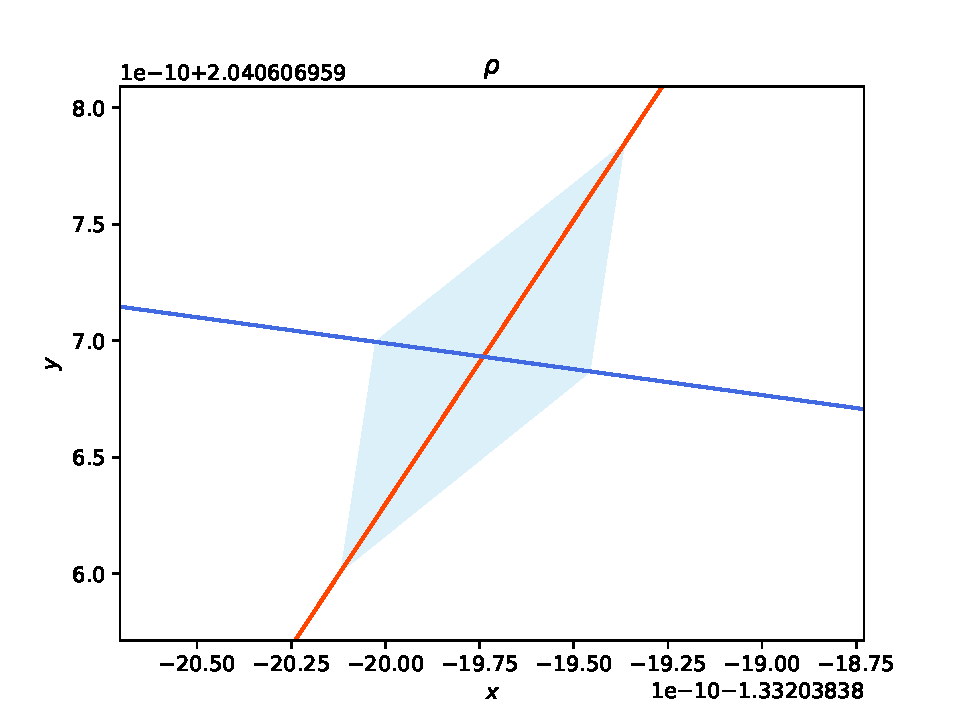
\includegraphics[width=65mm]{rho}}\hspace{0mm}
\subfigure{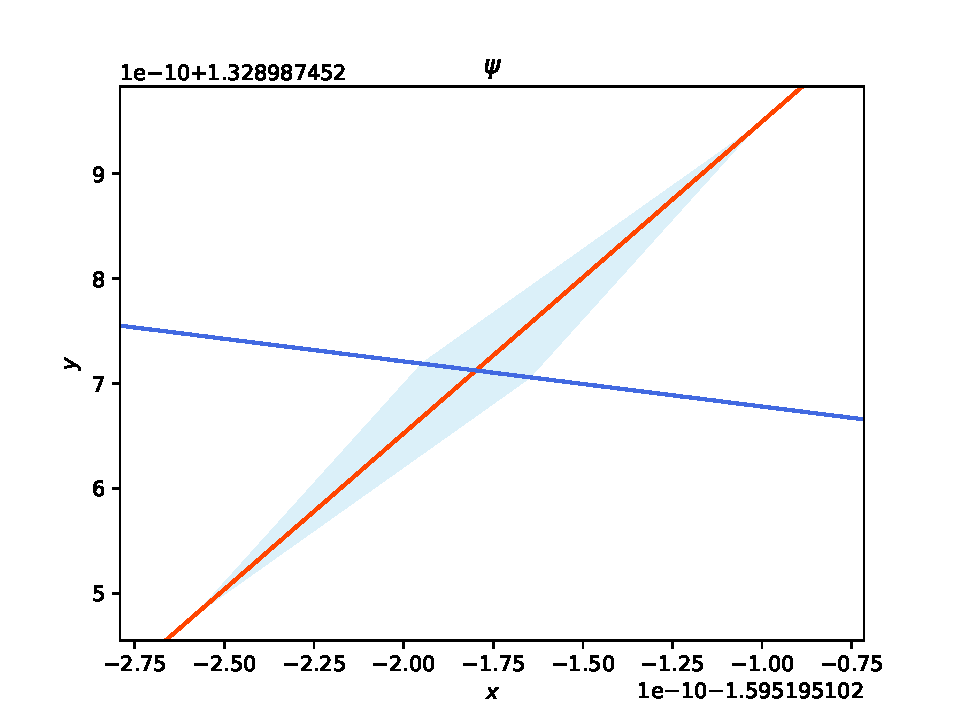
\includegraphics[width=65mm]{psi}}\vspace{0mm}
\subfigure{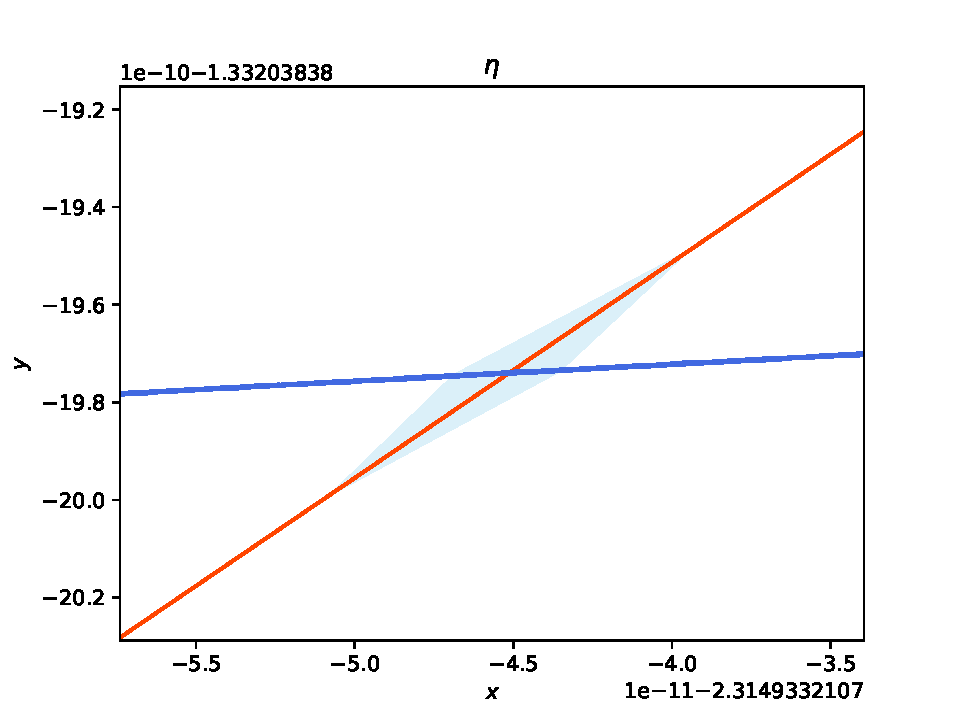
\includegraphics[width=65mm]{eta}}
\caption{Intervalos de intersecciones entre las variedades estable e inestable del mapeo de Hénon.} \label{matriz_cortes}
\end{figure}










La zona rectangular sombreada en cada gráfica representa el producto cartesiano de los intervalos donde se encuentra la solución. Es posible observar que de hecho cada zona contiene el cruce de las variedades, garantizando así que en el intervalo propuesto hay un cruce, siendo esta intersección punto homoclínico. Las regiones que aparecen en la figura \ref{matriz_cortes} son de área pequeña comparados con el área que ocupan las variedades. Este tipo de resultados son útiles para hablar sobre caos topológico \cite{devaney}, \cite{gerald}.\\

Para complementar este análisis se obtuvo una gráfica de las superficies que forman las variedades al cambiar el parámetro del mapeo, dando una idea de cómo se ven las superficies y además de cómo se comportan las intersecciones. La figura \ref{SuperficiesH} muestra las superficies formadas por las variedades para ciertos valores del parámetro $a$. Algunas gráficas más se encuentran en  \url{https://github.com/alvarezeve/Tesis-Variedades-Estables-e-inestables/} en el archivo llamado \texttt{Superficies.ipynb}.
\begin{figure}[H]
\centering
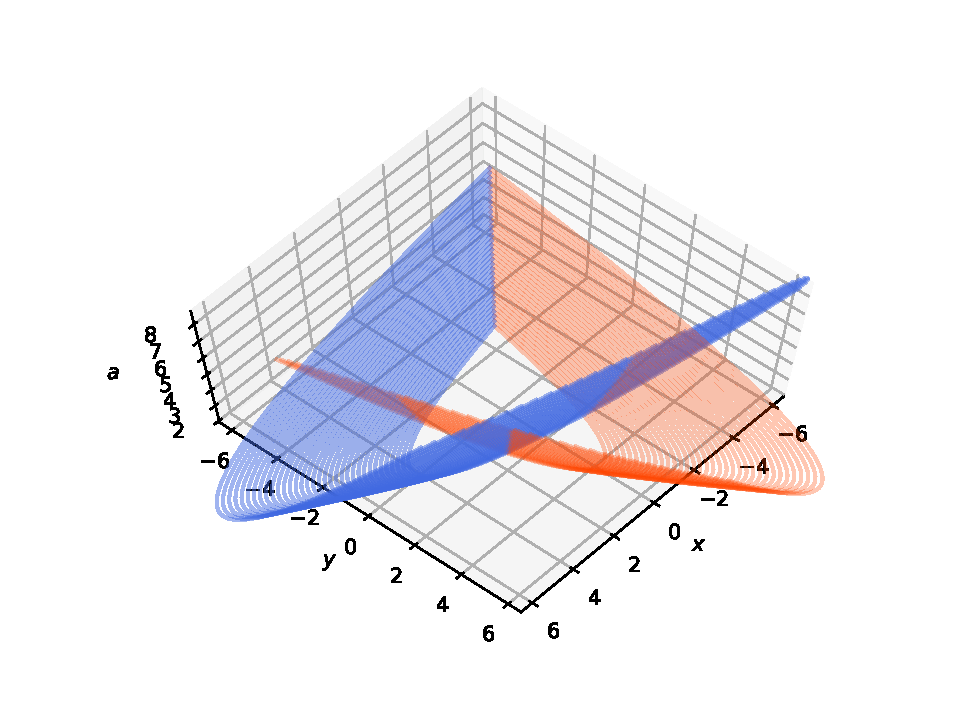
\includegraphics[scale=0.9]{HenonV}
\caption{Superficies en el mapeo de Hénon formadas por las variedades.}
\label{SuperficiesH}
\end{figure}



\subsection{Mapeo exponencial}
Las intersecciones en el caso del mapeo \eqref{Jung} se calcularon usando, como en los casos anteriores, el mapeo inverso \eqref{jungI}. Este mapeo representa un mayor reto en cuanto al orden del polinomio, pues la presencia de la exponencial hace que la parametrización sea sensible al orden del mismo. Para el siguiente ejemplo se utilizó un polinomio de orden 86 y una tolerancia en el método de Newton de $10^{-6}$ y se calcularon los cruces de las variedades como en los otros casos. Las siguientes fueron las secciones en términos del parámetro $t,\tau$ dónde se encontraron los cortes:
\begin{itemize}
\item[$\alpha$)] $[-0.985068, -0.985067] \times [5.99488, 5.99489]$
\item[$\beta$)] $[-3.46215, -3.46214] \times [5.49229, 5.4923]$
\item[$\gamma$)] $[-3.77896, -3.77895] \times [1.56269, 1.5627]$
\end{itemize}
La representación de los cortes se puede ver en la figura \ref{jung_cortes}.
\begin{figure}[H]
\centering
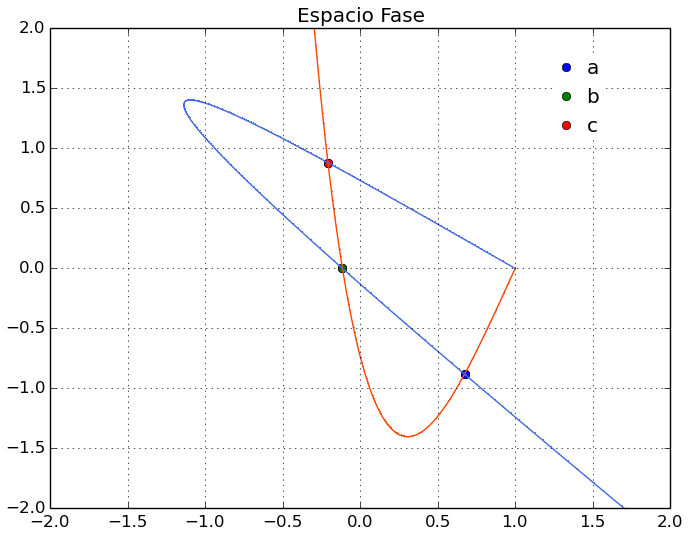
\includegraphics[scale=0.7]{cruces_jung1}
\caption{Intersecciones en el mapeo exponencial con $a=5.7$.}
\label{jung_cortes}
\end{figure}

Tomando los cruces a escala del intervalo se obtuvieron las figuras \ref{cruces_jung}.

\begin{figure}[htbp]
\centering
\subfigure{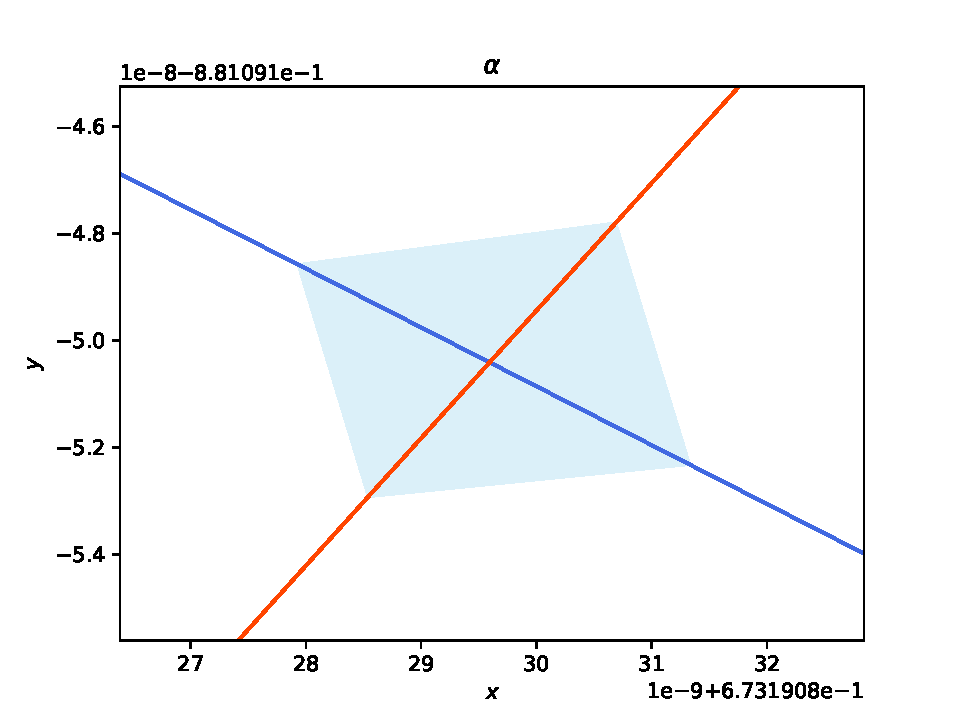
\includegraphics[width=80mm]{cruce_a}}
\subfigure{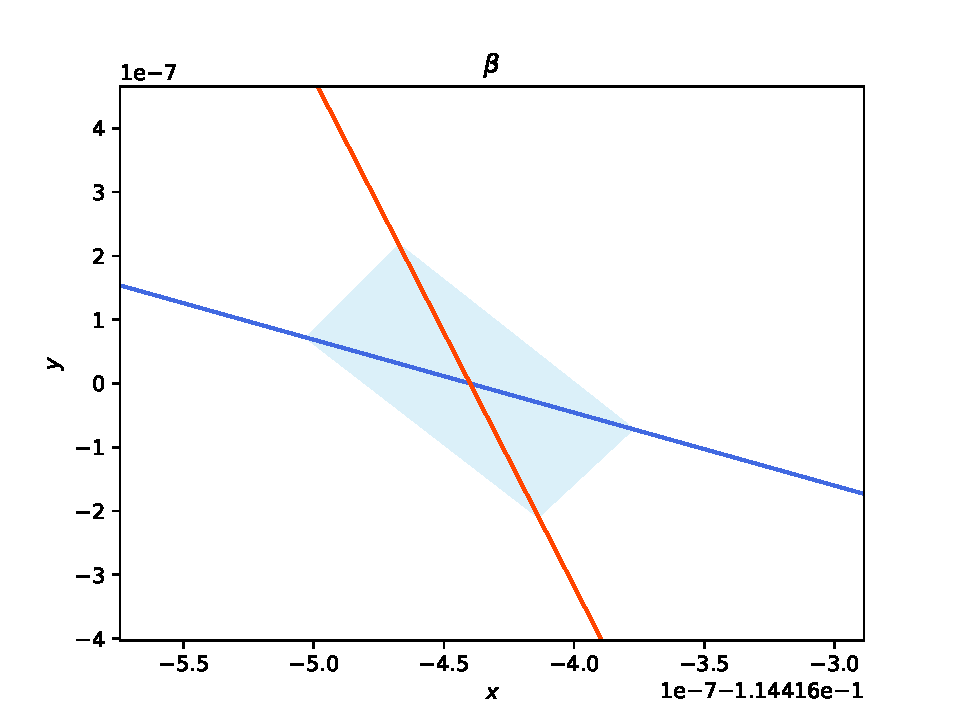
\includegraphics[width=80mm]{cruce_b}}
\subfigure{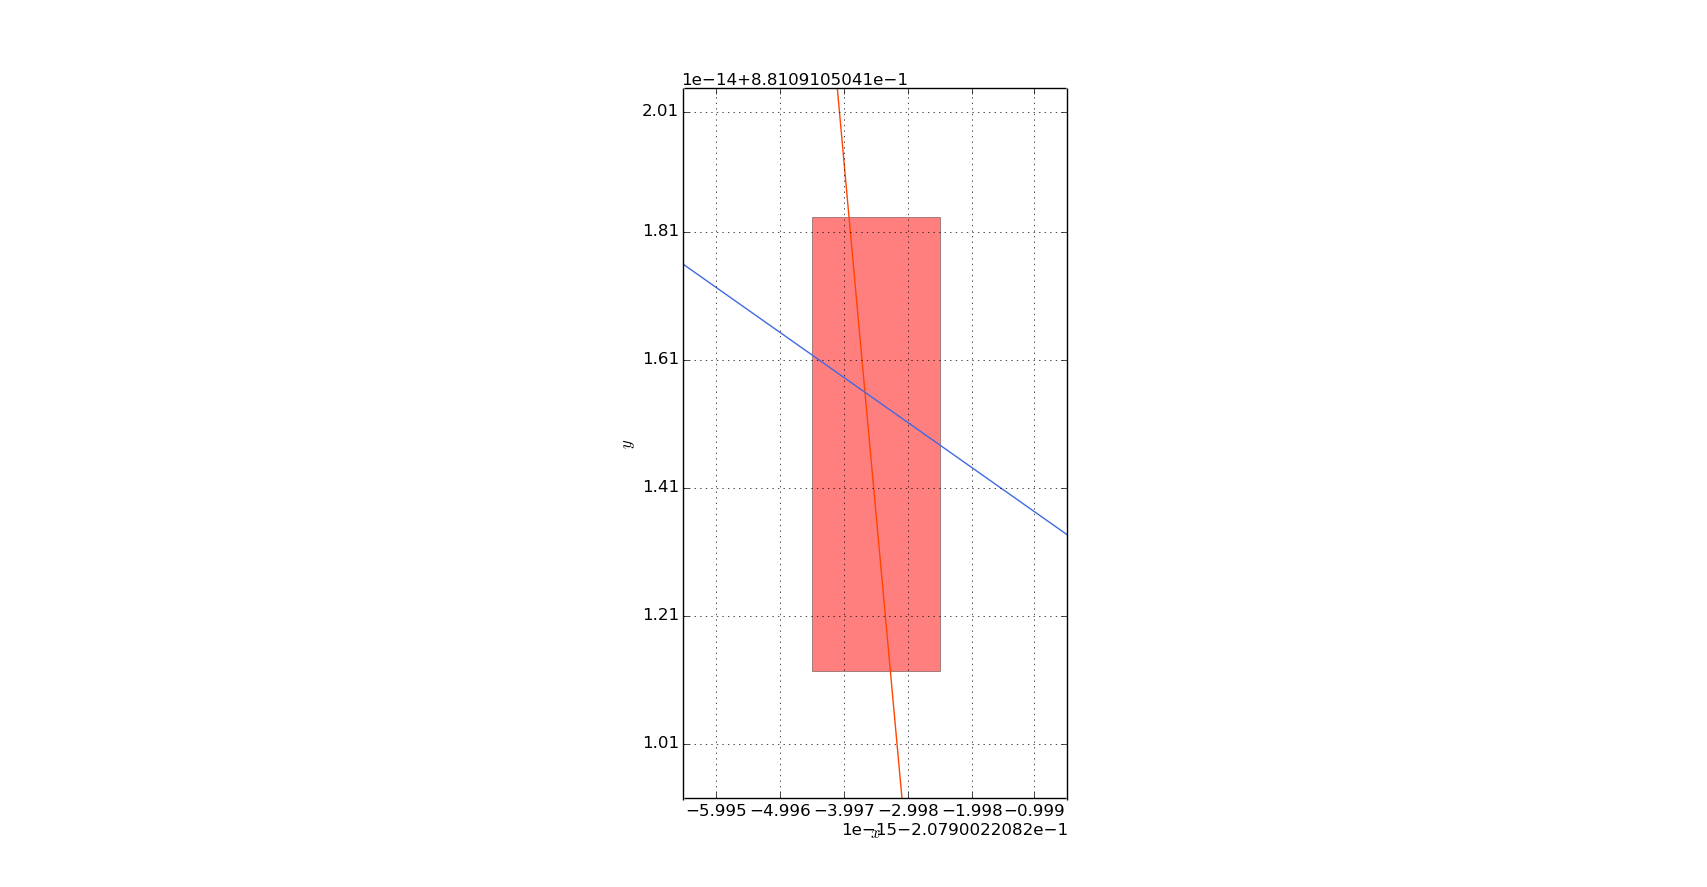
\includegraphics[width=80mm]{cruce_c}}
\caption{Intervalo de intersección de las variedades estable e inestable en el mapeo exponencial.} \label{cruces_jung}
\end{figure}




Las escalas en las que se observan los cortes de las variedades son pequeños com\-pa\-ra\-dos con la escala del mapeo, tanto que si se graficaran en el espacio fase no se podrían observar. Como ya se mencionó, ésto garantiza que existen tres puntos homoclínicos en el intervalo usado. \\
\linebreak
\linebreak
\linebreak
\linebreak
\linebreak
\linebreak
\linebreak
\linebreak


\label{SeccionRectanguloFundamental}\section{Rectángulo fundamental}
Para los mapeos abiertos como lo son Hénon y el mapeo de la sección anterior \ref{jung-seccion} se puede tener el \textit{rectángulo fundamental} a partir de los polinomios que se obtienen en el método de parametrización. El rectángulo fundamental es una región del espacio fase que contiene todas las intersecciones (homoclínicas y heteroclínicas) del mapeo, lo que permite obtener toda la dinámica fuera del mismo. Lo que pasa dentro del área del rectángulo fundamental con las variedades estables e inestables es una ventana a escala de lo que pasa si se extienden las variedades. A partir de esto se observan tentáculos o herraduras en la dinámica del mapeo; en la figura \ref{herradura} se muestra un diagrama de este tipo de comportamiento.

\begin{figure}[H]
\centering
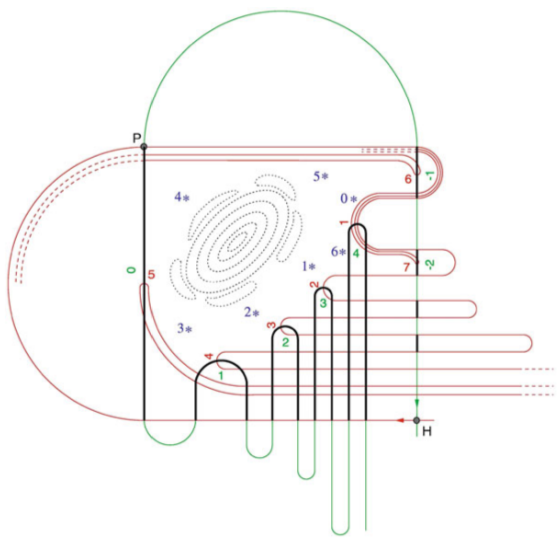
\includegraphics[scale=0.35]{herradura}
\caption{Diagrama ilustrativo de la topología de una herradura en un sistema Hamiltoniano de dos dimensiones. H denota el punto fijo hiperbólico y P la primera intersección. Los tentáculos de la variedad estable son enfatizados con color negro. Tomada de \cite{Merlo}, pp.8.}
\label{herradura}
\end{figure}

Una manera de llegar a observar estas estructuras con los polinomios de la pa\-ra\-me\-tri\-za\-ción sería usando polinomios de ordenes grandes; sin embargo como se ve en la gráfica \ref{erroresf64} de la sección \ref{SeccionEstandar} aumentar en 60 el orden del polinomio (de 20 a 80) sólo se traduce en una unidad del parámetro $t$ donde el error es mínimo. Para evitar calcular polinomios de órdenes grandes se toma la idea de la órbita de un punto, aplicando el mapeo a la parametrización, pues ésta representa los puntos sobre la variedad. Con esta idea se pudo encontrar parte de las estructuras mostradas en la figura \ref{herradura}, para los mapeos \eqref{Henon}, \eqref{Jung}.


En el caso del mapeo de Hénon con $a=6.5$ se calcularon polinomios de orden 250 usando números de precisión extendida ($W_{0}^{s},W_{0}^{u}$), además calcular la variedad estable usando el mapeo de Hénon inverso \eqref{HenonI}. En este caso se necesitó un valor máximo del parámetro $t=100$ para obtener el rectángulo fundamental, que se muestra en la figura \ref{rectangulo0}; en este caso, el error es menor a $10^{-73}$.

\begin{figure}[H]
\centering
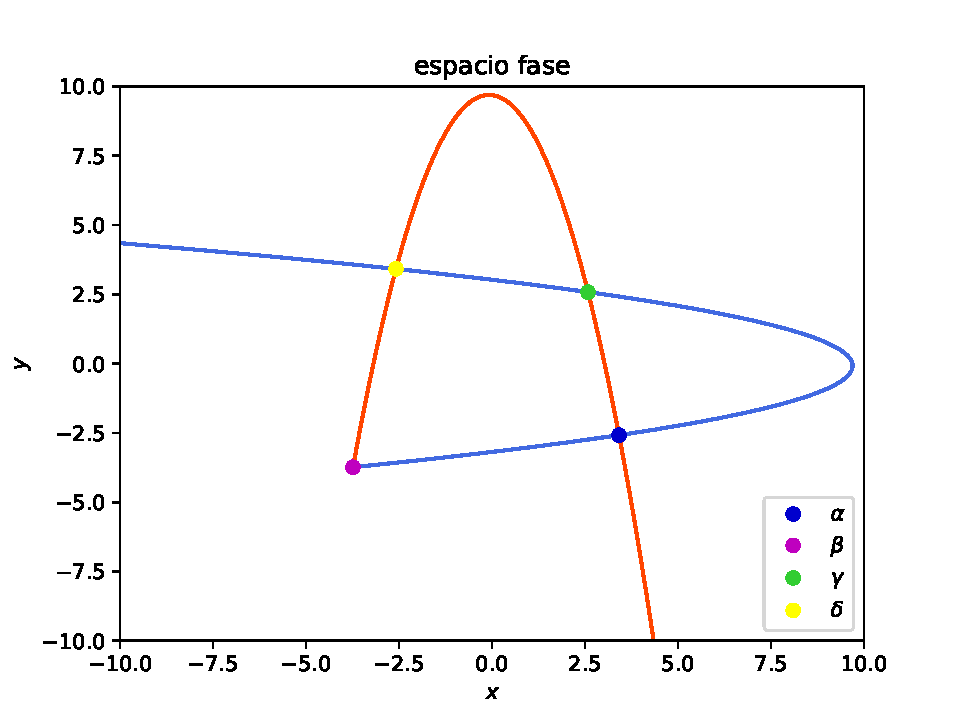
\includegraphics[scale=0.7]{rectangulo_fundamental}
\caption{Variedades estable e inestable de orden 250, para el mapeo de Hénon con $a=6.5,b=1.$, en el intervalo $t=[0.,100.]$. El punto $\omega$ denota el punto fijo mientras que $\alpha, \beta, \gamma$ son las primeras intersecciones de las variedades.}
\label{rectangulo0}
\end{figure}

\begin{figure}[H]
\centering
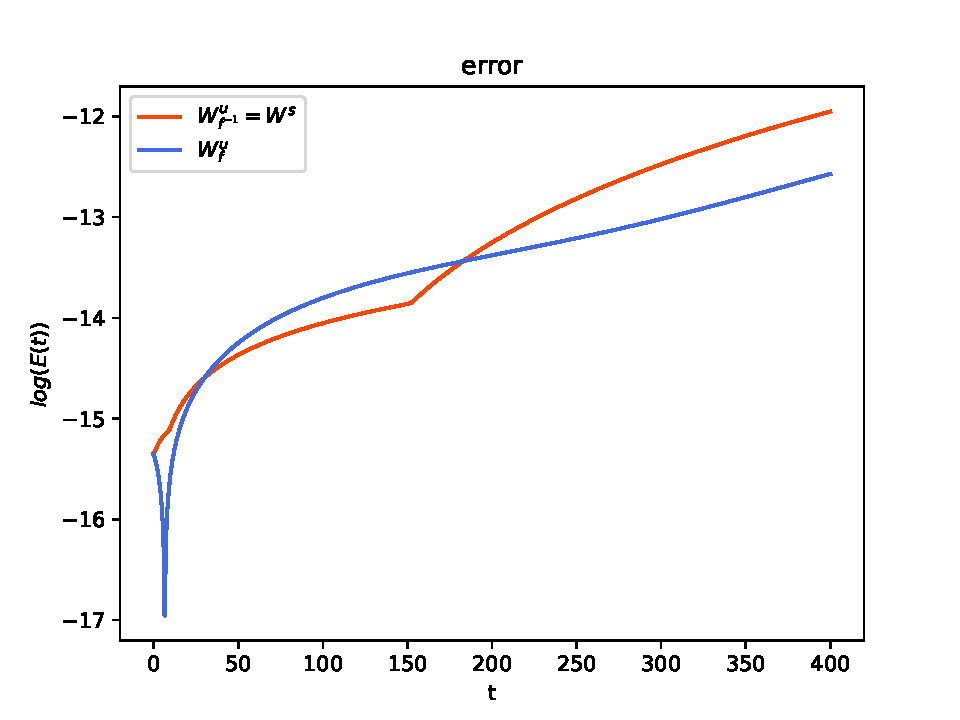
\includegraphics[scale=0.7]{error_rectangulo}
\caption{Error asociado al cálculo de las variedades en la figura \ref{rectangulo0}}.
\label{ErrorRectangulo0}
\end{figure} 

Reescribiendo la ecuación de invariancia \eqref{Ecua de invariancia} para el caso de la variedad estable, se obtiene:
\begin{eqnarray}
f_{a,b}^{-1}(W_{0}^{s}(t))=W_{0}^{s}(\lambda^{s}t).
\label{InvarianciaEstable1}
\end{eqnarray}

Aplicando el mapeo de Hénon inverso \eqref{HenonI} a la ecuación \eqref{InvarianciaEstable1} resulta
\begin{eqnarray}
W_{0}^{s}(t)=f_{a,b}(W_{0}^{s}(\lambda^{s}t)),
\label{InvarianciaEstable2}
\end{eqnarray}
que se reescribe como \eqref{InvarianciaEstable2}, 
\begin{eqnarray}
W_{0}^{s}\left(\frac{t}{\lambda^{s}}\right)=f_{a,b}(W_{0}^{s}(t)).
\label{InvarianciaEstable3}
\end{eqnarray}

Siendo que $\vert \lambda^{s} \vert < 1 $ la ecuación \eqref{InvarianciaEstable3} muestra que aplicar el mapeo es análogo a tener la variedad estable evaluada en un valor mayor del parámetro, puesto que $1/\lambda^{s}>1$. Este resultado es análogo para la variedad inestable. Usando esto se obtiene la figura \ref{Rectangulo1}, que muestra el resultado de iterar una vez, $(W_{x1}^{s},W_{y1}^{s})=f_{a,b}(W_{x}^{s},W_{y}^{s})$, análogamente para las inestables, evaluando los nuevos polinomios exactamente en los mismos intervalos que en el caso de la figura \ref{rectangulo0}.
\begin{figure}[H]
\centering
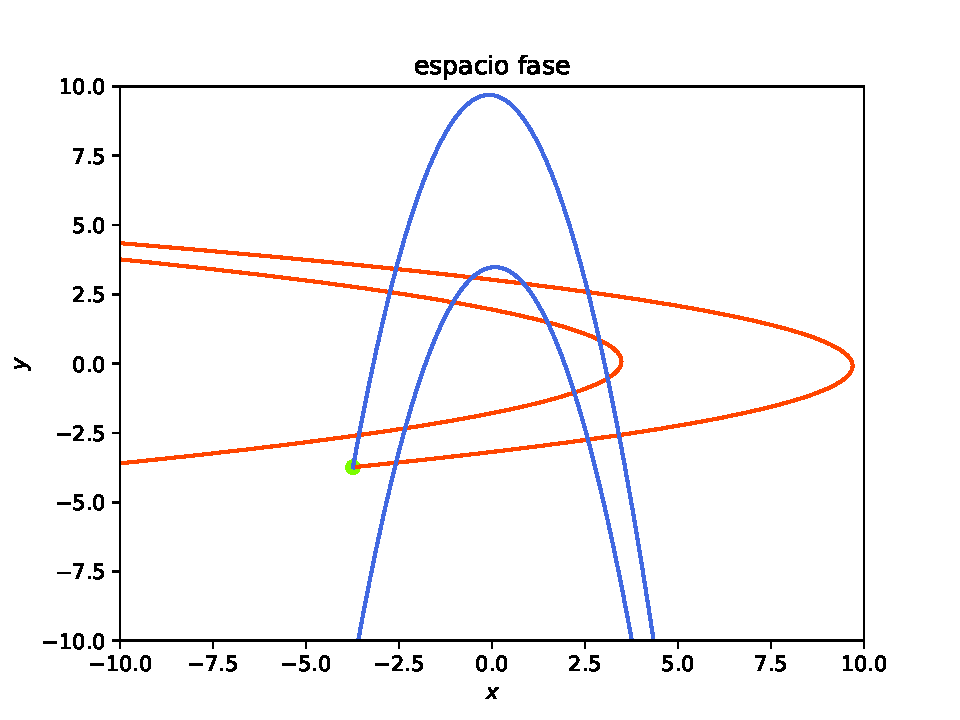
\includegraphics[scale=0.7]{rectangulo1.pdf}
\caption{Primera aplicación del mapeo a los polinomios de orden 250, $t=[0,100]$.}
\label{Rectangulo1}
\end{figure}
El cálculo con el que se obtiene la figura \ref{Rectangulo1} produce un nuevo polinomio el cual tiene asociado también un error numérico. Para saber cuál es este error se usó la ecuación \eqref{InvarianciaEstable3},
\begin{eqnarray}
E_{1}(t)=\bigg\| W_{0}^{s}\left(\frac{t}{\lambda^{s}}\right)-f_{a,b}(W_{0}^{s}(t))\bigg\|_{\infty},
\label{error-1aplicacion}
\end{eqnarray}
está forma es análoga a la ecuación \eqref{Ecua de invariancia resta}, la cual se representa en la figura \ref{error-1iteracion}. De la misma manera se evalúa el error en las aplicaciones consecutivas, el cual se expresa como
\begin{eqnarray}
E_{n}(t)=\bigg\| (f^{-1}_{k})^{n}\left(W_{0}^{s}\left(\frac{t}{\lambda^{s}}\right)\right)- (f^{-1}_{k})^{n-1}(W_{0}^{s}(t)))\bigg\|_{\infty}.
\label{error-n-aplicacion}
\end{eqnarray}
En la ecuación \eqref{error-n-aplicacion} $n$ representa el número de aplicaciones del mapeo, mientras que $W_{0}$ es la parametrización inicial calculada mediante el método.\\

\begin{figure}[h!]
\centering
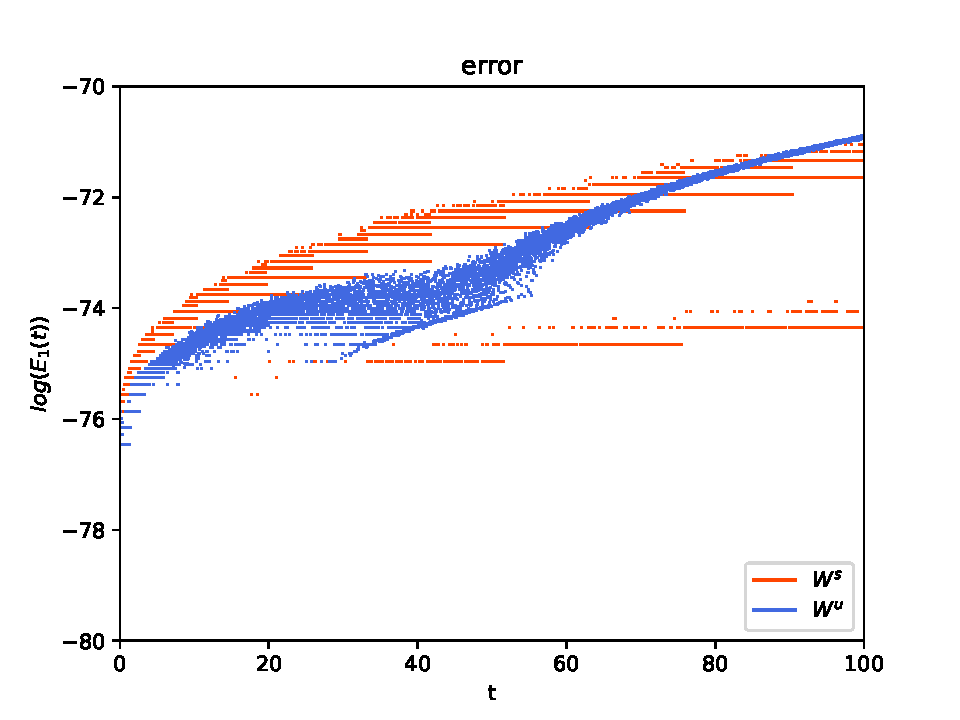
\includegraphics[scale=0.7]{error1ite.pdf}
\caption{Error en el polinomio que resulta de aplicar el mapeo a la parametrización de orden 250.}
\label{error-1iteracion}
\end{figure}
Se puede observar en la figura \ref{error-1iteracion} que el error es mínimo en ambas variedades, manteniéndose por debajo del orden de $10^{-70}$; las líneas verticales son producto de valores numéricos que aparecen como cero al evaluar el polinomio a los cuales se les sumó un valor del orden de $10^{-120}$ para poder evaluar el logaritmo base $10$ del error. Al revisar en la sección \ref{henon-seccion}, el error crece mucho más rápido cuando sólo se usa el polinomio que resulta de la parametrización, además de que no es posible llegar tan lejos como se muestra en las figuras \ref{Rectangulo1}-\ref{Rectangulo5}.\\

La segunda aplicación del mapeo a los polinomios, $(W_{x2}^{s},W_{y2}^{s})=f_{a,b}(W_{x1}^{s},W_{y1}^{s})$ se muestra en la figura \ref{Rectangulo2}, de nuevo usando el mismo valor máximo del parámetro $t$, además en la figura \ref{error-2iteracion} muestra el error asociado a tal resultado.\\
\begin{figure}[h!]
\centering
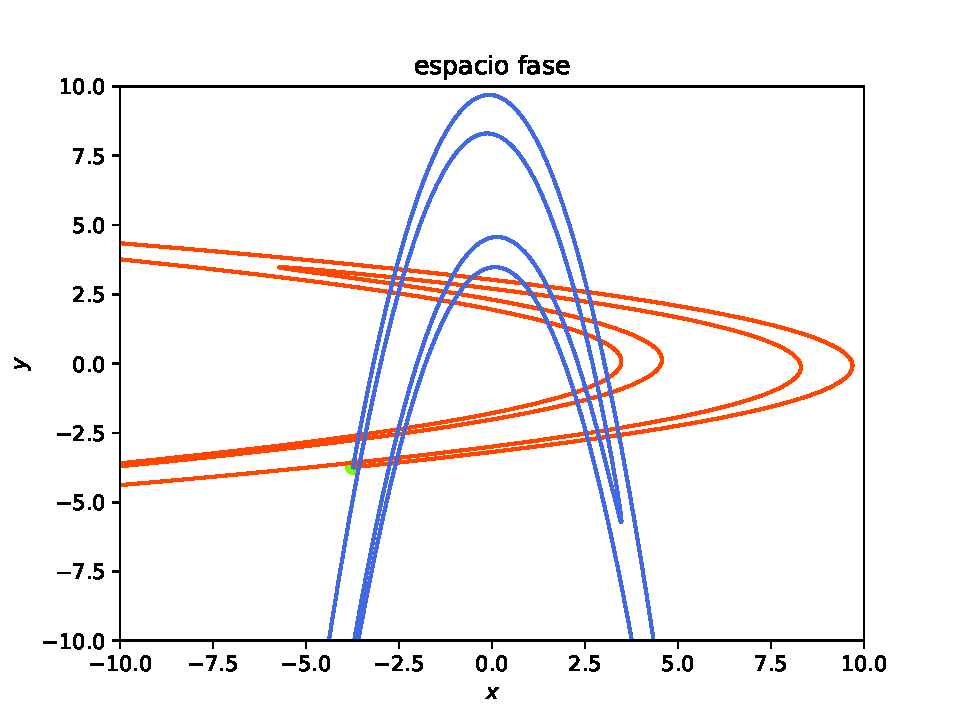
\includegraphics[scale=0.7]{rectangulo2.pdf}
\caption{Segunda aplicación del mapeo a los polinomios de orden 250.}
\label{Rectangulo2}
\end{figure}

\begin{figure}[h!]
\centering
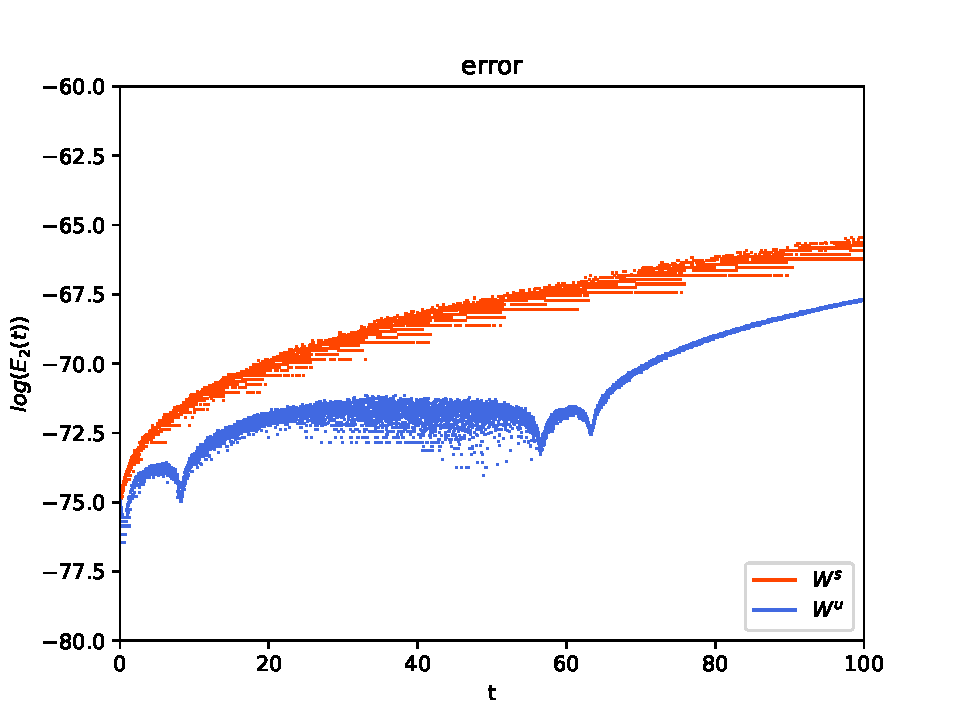
\includegraphics[scale=0.7]{error2ite.pdf}
\caption{Error en el polinomio que resulta de aplicar el mapeo por segunda vez a la parametrización de orden 250.}
\label{error-2iteracion}
\end{figure}

De manera sucesiva se aplicaron los mapeos correspondientes hasta iterar cinco veces, siempre conservando el mismo valor máximo del parámetro $t$.
\begin{figure}[h!]
\centering
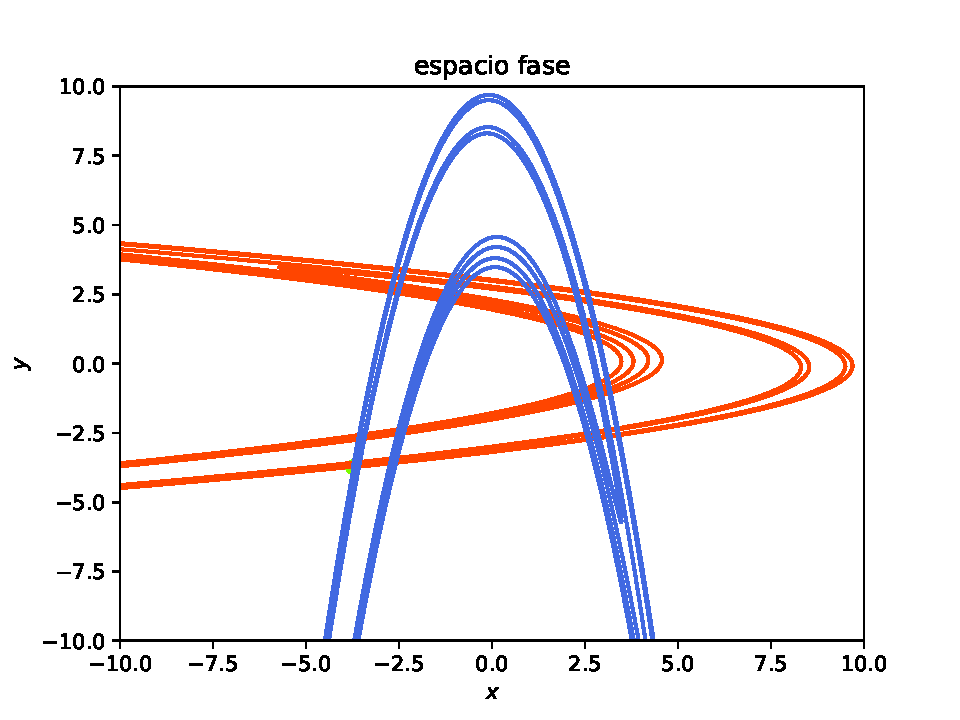
\includegraphics[scale=0.7]{rectangulo3.pdf}
\caption{Tercer aplicación del mapeo a los polinomios de orden 250.}
\label{Rectangulo3}
\end{figure}

\begin{figure}[h!]
\centering
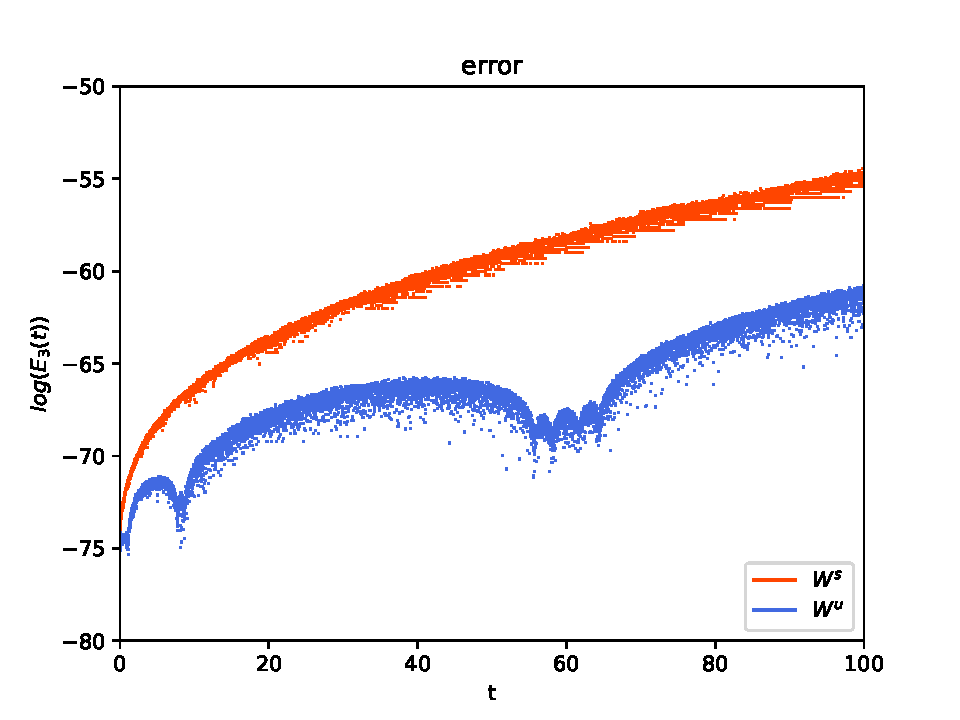
\includegraphics[scale=0.7]{error3ite.pdf}
\caption{Error en el polinomio que resulta de aplicar el mapeo por tercera vez a la parametrización de orden 250.}
\label{error-3iteracion}
\end{figure}

\begin{figure}[h!]
\centering
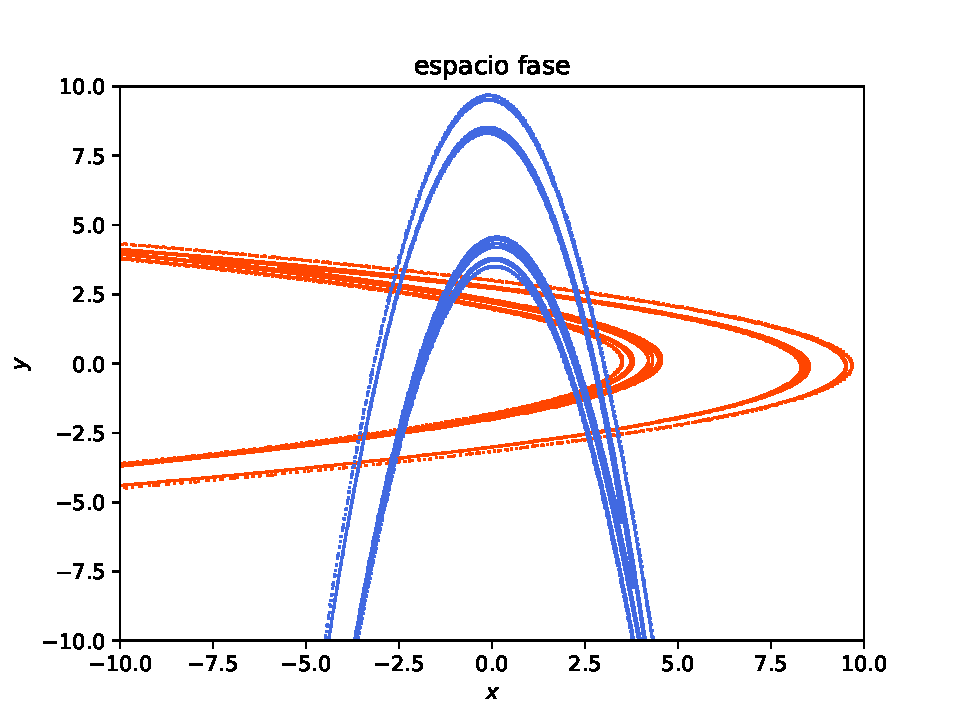
\includegraphics[scale=0.7]{rectangulo4.pdf}
\caption{Cuarta aplicación del mapeo a los polinomios de orden 250.}.
\label{Rectangulo4}
\end{figure}

\begin{figure}[h!]
\centering
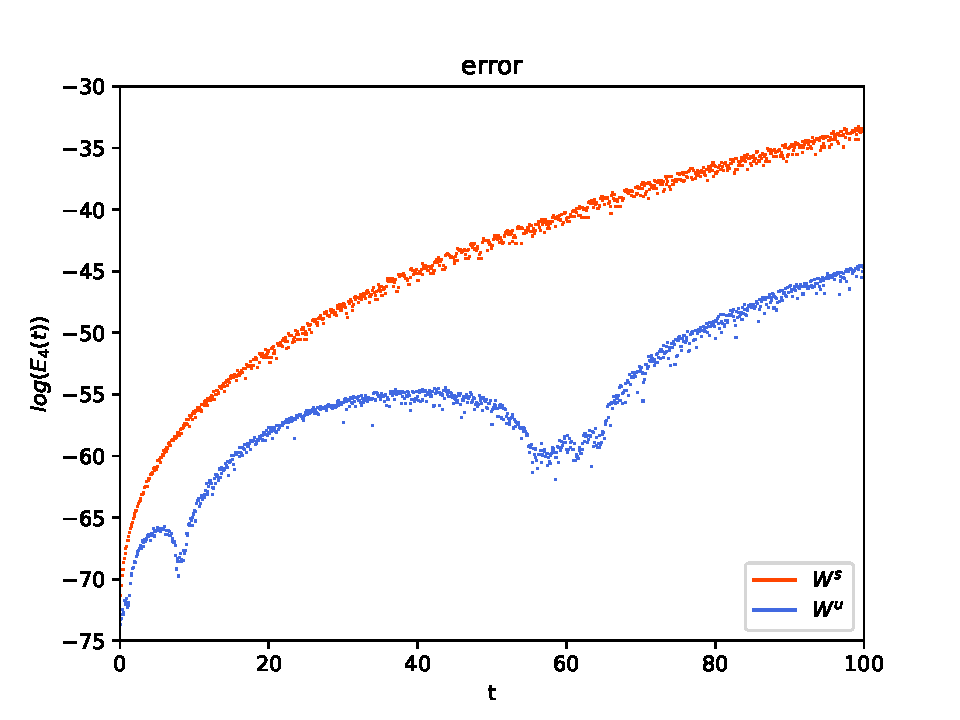
\includegraphics[scale=0.65]{error4ite.pdf}
\caption{Error en el polinomio que resulta de aplicar el mapeo por cuarta vez a la parametrización de orden 250.}
\label{error-4iteracion}
\end{figure}

\begin{figure}[H]
\centering
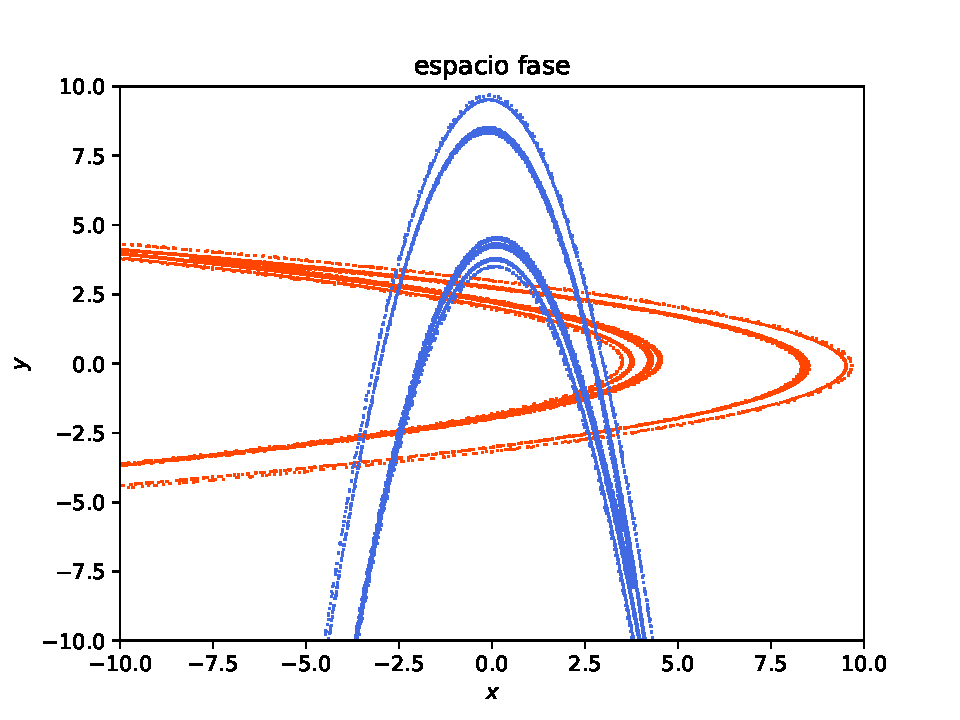
\includegraphics[scale=0.7]{rectangulo5.pdf}
\caption{Quinta aplicación del mapeo a los polinomios de orden 250.}.
\label{Rectangulo5}
\end{figure}

\begin{figure}[H]
\centering
\includegraphics[scale=0.7]{error5ite.pdf}
\caption{Error en el polinomio que resulta de aplicar el mapeo por quinta vez a la parametrización de orden 250.}
\label{error-5iteracion}
\end{figure}

En las primeras dos aplicaciones del mapeo, \ref{Rectangulo2} y \ref{Rectangulo3}, se puede observar un tentáculo más en cada variedad, mientras que en las siguientes aparecen hasta dos más. La profundidad de tentáculos y la forma en la que se cruzan depende del valor del parámetro $a$. Hay que enfatizar que para lograr observar estos cruces de manera directa, se debería llegar a valores del parámetro muy grandes comparados con el valor que se usó en todos los casos, lo cual no siempre es posible, pues como se vio en la sección \ref{SeccionEstandar} después de cierto orden el error se estanca y no es posible llegar tan lejos con errores controlables, mientras que como muestran las figuras \ref{error-1iteracion}-\ref{error-4iteracion} el error es mucho menor que si se usara un polinomio de orden grande $(>250)$. Con esto es evidente que sólo se necesita conocer el rectángulo fundamental para conocer mucho de la dinámica de las variedades, y por tanto de los cruces entre ellas.\\ 


La implementación del método resultó ser eficiente para encontrar los polinomios que representan las variedades estable e inestable asociadas a puntos fijos hiperbólicos de los diferentes mapeos. Se tomaron estos tres mapeos para tener un poco de variedad en la forma de las variedades y también de los puntos fijos. En todos los casos el orden de la parametrización afecta de manera diferente: para el caso del mapeo exponencial resulta ser más sensible. En todos ellos un orden mayor contribuye a llegar más lejos en el valor del parámetro con un error bajo y como consecuencia graficar de mejor manera las variedades. El error se manipula al mover el orden pero también, se puede mejorar al usar números de precisión extendida. Una característica que se puede observar es que el error se comporta esencialmente de la misma forma para los tres mapeos, creciendo de manera lenta y luego creciendo rápido a partir de cierto valor. \\


El análisis de la convergencia resulta congruente con lo que se puede observar en el error y en las mismas gráficas de las variedades. La convergencia también ayudó a ver que a partir de cierto orden los coeficientes son muy pequeños, por lo que no es necesariamente cierto que cada que aumente el orden se mejorará la parametrización.\\


El cálculo de puntos homoclínicos resulta una de las aplicaciones de tener las variedades parametrizadas. El método, junto con otras paqueterías de Julia, son in\-dis\-pen\-sa\-bles para hacer este tipo de cálculos de una manera fácil. A pesar de que la aritmética de intervalos arroja resultados garantizados, no hay que olvidar que nuestros polinomios no son calculados de la misma manera, es decir se debe tener siempre en mente que alrededor de cada variedad hay un error asociado. Aún así las intersecciones pueden ser encontradas controlando bien el error en la parametrización y controlando la tolerancia en el método de Newton.